
% -----------------------------------------------------------------------
% Python Tutorial
% WS 18/19
% -----------------------------------------------------------------------
\documentclass[enabledeprecatedfontcommands, fontsize=12pt,
     open=right, a4paper,
     twoside, DIV=11,
     abstractoff,
     headsepline,
     numbers=noenddot,
     BCOR=15mm,
     headings=standardclasses,
     headings=big]{scrbook}
\KOMAoptions{cleardoublepage=empty}
% Header f�r Variablen
% Variablen
\newcommand{\theSemester}{Sommersemester 2019}
% Variable f�r die Vorlesung
\newcommand{\theProject}{}
% Variable f�r den Studiengang
\newcommand{\theTitle}{Python}
% Variable f�r den Hochschul-Namen
\newcommand{\theSchool}{Hochschule Kaiserslautern}
% Variable f�r den Dozenten
\newcommand{\theAuthor}{
    Julian  Bernhart,
    Manfred Brill,
    Eric Brunk,
    Mathias Fedder,
    Christopher Gross,
    Robin Guth,
    Rainer Haffner,
    Matthias Haselmaier,
 %   Kathrin Hentschel,
    Fabian Kalweit,
    Lukas Kuhn,
    Kevin Konrad,
    Philipp Lauer,
    Miriam Lohm�ller,
    Sebastian Morsch,
    Anatoli Sch�fer,
    Denis Schlusche,
    Christoph Seibel,
    Marc Zintel
}

%
% ----------------------------------------------------------------------------------------------
% Vorlage f�r Dokumentation auf LaTeX-Basis im Projekt InfoStuDi
% --------------------------------------------------------------------------------------------
\usepackage{mb}
\usepackage{mbmath}
\usepackage{textcomp}
\usepackage{german}
% Array-Paket f�r mehr Kontrolle der Tabellen
\usepackage{array}
% ifthen f�r Ein- und Ausblenden der L�sungen.
\usepackage{ifthen}
% Paket f�r Postscript Pi-Fonts
\usepackage{pifont}
% PSTricks
%\usepackage{pstricks}
% Paket f�r das einfache Umdefinieren von Listen
\usepackage[shortlabels]{enumitem}
% Alphabetischer Index
\usepackage{imakeidx}
\makeindex[title=Index,columns=2,options=-s german,intoc]
% Header und Footer mit KomaScript
\usepackage[automark, headsepline]{scrlayer-scrpage}
% Caption unteraderm, dass \ref nicht nur zur Caption sondern auch zur Figure springt
\usepackage{caption}
%
% Header f�r Werkzeuge, Begriffe aus dem Software-Management
\input{variablen}
% Farben
\input{colors}
% Standardverzeichnis f�r das Basisverzeichnis der Bilder
%
\newcommand{\imagePath}{./images}
%
\raggedbottom
\setlength{\parskip}{2.0ex}
\setlength{\parindent}{0.0cm}
%% Verhindert Schusterjungen und Hurenkinder
\clubpenalty = 10000
\widowpenalty = 10000 \displaywidowpenalty = 10000
%
\setcounter{secnumdepth}{2}
\setcounter{tocdepth}{2}
%
\pagestyle{scrheadings}
\clearscrheadfoot
% Thema des Dokuments in die Kopfzeile
\ihead{\headmark}
\ohead[]{\pagemark}
\chead{}
\pagestyle{scrheadings}
% Abst�nde zwischen Caption und Bild/Tabelle
\setlength\abovecaptionskip          {0.4em}
\setlength\belowcaptionskip          {0.2em}
% Anteil der Grafiken h�her auf jeder Seite!
\renewcommand{\textfraction}{0.001}
\renewcommand{\topfraction}{0.99}
% Literatur-Stil
\bibliographystyle{geralpha}
% Listingspaket
\usepackage{listings}
\lstloadlanguages{python}
\lstset{language=python}
\definecolor{lstback}{gray}{0.85}
\lstset{backgroundcolor=\color{lstback}}
\lstset{extendedchars=true}
\lstset{showstringspaces = false}
\lstset{basicstyle = \ttfamily \small}
%% listings mit listings.sty
%
% Kommando f�r den Flattersatz bei nebeneinander liegenden Abbildungen
\newcommand{\flatter}{\setlength{\rightskip}{0pt plus 2cm}}
%
% Schritte in einer Aufz�hlung, daf�r einen Z�hler (schritt) und die Umgebung
% schritte definieren.
\newcounter{schritt}
\newenvironment{schritte}%
{\begin{list}%
{Schritt \arabic{schritt}:}%
{\usecounter{schritt}\settowidth{\labelwidth}{Schritt 1:}%
\setlength{\leftmargin}{\labelwidth}\addtolength\leftmargin{\labelsep}%
\parsep0.0ex\partopsep-0.3ex\itemsep2pt\topsep0.0ex}}{\end{list}}
% Dateinamen f�r interne Musterl�sungen
\newcommand{\filename}[1]{%
\ifthenelse{\boolean{solutions}}{\framebox[50mm]{\parbox{40mm}{\textbf #1}}\vspace{6pt}}{}}
%   Taste
\newcommand{\taste}[1]{\small\textsf{#1}\normalsize}
%   gesch�tzte Namen (NICHT in chapter, section usw. verwenden!)
\newcommand{\name}[1]{\textsl{#1}}
%   Fachbegriffe/Erkl�rung von Abk�rzungen
\newcommand{\begriff}[1]{\index{#1}\textit{#1}}
%
\newcommand{\algorithmus}[2]{%
\vspace{4pt}\fboxsep 1mm \framebox[140mm]
{\parbox{135mm}{{\textbf{#1}}\vspace{2pt}#2}}\vspace{4pt}}
%
%   Dateinamen/Pfade
\newcommand{\datei}[1]{\texttt{#1}\normalsize}
%   Tip (in einer Box)
\newcommand{\tip}[1]{%
\vspace{4pt}\fboxsep 1mm \framebox[140mm]
{\parbox{135mm}{{\textbf{Tipp}}:\\ #1}}\vspace{4pt}}

%Achtung in einer Box
\newcommand{\warning}[1]{%
    \par\vspace{4pt}\fboxsep 1mm \framebox[140mm]%
    {\parbox{135mm}{{\textbf{Achtung}}:\\ #1}}\vspace{4pt}%
}
%

%
%   Reflektion (in einer Box)
%
\newcommand{\reflection}[1]{
\begin{quote}\fboxsep 3mm\framebox[140mm][c]{\parbox{130mm}{{\textbf{Reflektion}:\\}#1}}\end{quote}}
%
%   Angabe, was die Studierenden lesen sollen (in einer Box)

\newcommand{\lesen}[1]{%
\begin{minipage}[c]{2.5cm}
\centering
\includegraphics[width=2cm]{\imagePath/Misc/buchicon}%
\end{minipage}%
\begin{minipage}[t]{12cm}%
#1%
\end{minipage}}
%
%   Angabe im Begleittext, was die Studierenden lesen sollen (in einer Box)
%   Dieses Icon wird f�r Angaben verwendet, die nicht verpflichtend zu lesen
%   sind. Also "nice-to-have", "wenn sie noch Zeit haben".
\newcommand{\vertiefen}[1]{%
\begin{minipage}[b]{2.5cm}
\centering
\includegraphics[width=2cm]{\imagePath/Misc/reading}%
\end{minipage}%
\begin{minipage}[b\newcommand{\firefox}{\texttt{Mozilla Firefox}}
\newcommand{\kde}{\texttt{KDE}}]{12cm}%
#1%
\end{minipage}}
%
% Jetzt kommt die Definition der Kontrollfrage; die Nummerierung
% f�r das ganze erhalten wir mit Hilfe von \item{\kontroll}.
%
% Ein Counter f�r die Kontrollfragen. Wir z�hlen diesen Counter selbst hoch
% mit einem entsprechenden Kommando, das wir in \item verwenden.
% 1
\newcounter{kontrollCounter}[section]
\newcommand{\kontroll}[0]{
    \refstepcounter{kontrollCounter}
    % Kapitelnummer.Z�hler f�r das Item
    \arabic{chapter}.\arabic{kontrollCounter}
    % Das Label ist bis auf weiteres "kontrolle:Kapitelnummer:kontrollcounter
    \label{kontrolle:\arabic{chapter}:\arabic{kontrollCounter}}
}
% Jetzt kommt die Definition der Kontrollfrage; die Nummerierung
% f�r das ganze erhalten wir mit Hilfe von \item{\kontroll}.
\newcommand{\kontrollfrage}[1]{%
\begin{minipage}[c]{1.85cm}
\huge{\ding{46}}%
\end{minipage}%
\begin{minipage}[t]{12cm}%
\begin{itemize}#1%
\end{itemize}%
\end{minipage}}
%
% Einblenden von Musterl�sungen
%
% Schalter f�r das ein- und ausblenden der L�sungen
\newboolean{solutions}
%
% Theorem-Umgebung f�r die �bungsaufgaben
% Wichtig: alle Attribute einstellen, dann die neue
% theorem-Umgebung mit newtheorem definieren!
% Oder, wie hier, durch das Einschlie�en in {}
%
{
% Zeilenumbruch bei Aufgaben-�berschrift
\theoremstyle{break}
% "Normaler" Font im Text
\theorembodyfont{\normalfont}
% Kapitelweise neu nummerieren
% 2
\newtheorem{auftitle}{Aufgabe}[section]
}
%
% Definition f�r die Kennzeichnung der �bungsaufgaben
%
\newcommand{\uebung}{%
\vspace*{11pt}%
\begin{tabular}{@{}p{2.25cm}@{}p{11.7cm}}%
\huge{\ding{45}}&\Large{\textbf{�bungsaufgaben}}%
\end{tabular}%
}
% Ein Counter f�r die �bungsaufgaben. Wir z�hlen diesen Counter selbst hoch
% mit einem entsprechenden Kommando, das wir in \item verwenden.
% 3
\newcounter{aufgabenCounter}[section]
\newcommand{\auf}[0]{
    \refstepcounter{aufgabenCounter}
    % Kapitelnummer.Z�hler f�r das Item
    \arabic{chapter}.\arabic{aufgabenCounter}
}
% Der Text der Aufgaben steht im Ordner ./exercises/tasks/aufgabenstellungen,
% so k�nnen wir die Dateien aus der Veranstaltung
% Wahrscheinlichkeitsrechnung und Statistik verwenden; und die neuen
% Aufgaben gehen in den allgemeinen Fundus ein.
%

% Umgebungen f�r Satz, Definition, Beweis, ... . Wir orientieren uns am Mathematik-Buch,
% dort gab es diese Umgebungen auch schon. Im Grunde sind das einfach
% wieder theorem-Umgebungen.
{
\setlength\theorempreskipamount{5pt plus 3pt minus 1.5pt}
\setlength\theorempostskipamount{5pt plus 1pt minus 1pt}
% "Normaler" Font im Text
\theorembodyfont{\normalfont}
% Die Namen sind so gew�hlt, dass sie kompatibel zu Beamer sind; dann k�nnen
% wir den Text aus Folien kopieren und umgekehrt auch.
% 4
\newtheorem{Satz}{Satz}[section]
\newtheorem{Fakt}{Fakt}[section]
\newtheorem{Definition}{Definition}[section]
}
%
{
\setlength\theorempreskipamount{8pt plus 3pt minus 1.5pt}
\setlength\theorempostskipamount{5pt plus 1pt minus 1pt}
\theoremstyle{break}
% "Normaler" Font im Text
\theorembodyfont{\normalfont}
\newtheorem{datensatz}{Datensatz}
}
% Text mit Pfad
\newcommand{\aufgabentext}[1]{\renewcommand{\labelenumi}{\alph{enumi})}\auftitle\label{#1}\input{./exercises/tasks/#1} }
% Funktion f�r die L�sungs-Hinweise f�r eine Aufgabe. Der Text
% steht analog zu den �bungsaufgaben im Ordner tasks/solutions.
\newcommand{\hinweistext}[1]{\renewcommand{\labelenumi}{\alph{enumi})}\input{./exercises/solutions/#1}}
% Und jetzt die Funktionen, die wir im Text aufrufen
\newcommand{\aufgabe}[1]{\aufgabentext{#1}}
% L�sungshinweise im Anhang
\newcommand{\hinweis}[1]{\subsubsection*{Aufgabe \ref{#1}}\label{#1sol}  \hinweistext{#1}}
%
% Datensatz-Texte und Daten in eigener Datei
\newcommand{\dataset}[1]{\begin{datensatz}\label{#1}\input{./exercises/datasets/#1}\end{datensatz}}
% Teilaufgaben alphabetisch nummerieren
\renewcommand{\labelenumi}{\arabic{enumi})}
%
% Marginalien
%
\newcommand{\randnotiz}[1]{\marginpar{\small{\textbf{#1}}}}
%
% Gabelschl�ssel als Marginalie und Hinweis auf Praxisbezug
\newcommand{\praxisbezug}[0]{\randnotiz{\includegraphics[width=1cm]{\imagePath/Misc/gabel}}}
%
% alert aus beamer-Folien zu emph machen
%
\newcommand{\alert}[1]{\emph{#1}}
%
%
\newcommand{\titelseite}[1]{%
% Titelseite
\pagenumbering{roman}%
\thispagestyle{empty}%
\begin{titlepage}%
% Volle Zeilenbreite verwenden!
\centering%
\vspace*{2cm}%

\Huge{\textbf{#1}}\\\vspace*{0.5cm}%

\vspace*{10cm}%

\Large{\theAuthor{}}%

\Large{\theProject{}}%

\Large{\theSchool{}}%
\end{titlepage}}

% Titelseite mit zus�tzlicher Grafik
%
%
\newcommand{\titelseiteMitBild}[1]{%
%% Titelseite
\pagenumbering{roman}%
\thispagestyle{empty}%
\begin{titlepage}%
% Volle Zeilenbreite verwenden!
\centering%
\vspace*{0.5cm}%

\Huge{\textbf{#1}}\\\vspace*{0.5cm}%

\vspace*{2.0cm}%

\vspace*{1.0cm}%

\Large{\theProject{}}%

\Large{\theSchool{}}%

\vspace*{2.0cm}%

\normalsize{\theAuthor{}}%
\end{titlepage}}

%\makeatletter
%\newcommand{\shoppinglist}[1]{%
%   Shopping list: #1\checknextarg}
%\newcommand{\checknextarg}{\@ifnextchar\bgroup{\gobblenextarg}{ and that's all!}}
%\newcommand{\gobblenextarg}[1]{ and also #1\@ifnextchar\bgroup{\gobblenextarg}{ and that's all!}}
%\makeatother

\makeatletter
\newcommand{\templabel}{xxx}
\newcommand{\uebungTutorial}[1]{%
    \vspace*{11pt}%
    \begin{tabular}{@{}p{2.25cm}@{}p{11.7cm}}%
        \huge{\ding{45}}&\Large{\textbf{�bungsaufgaben}}%
    \end{tabular}%
    \aufgabe{#1}
    \renewcommand{\templabel}{#1sol}
    \checknextarg{#1}
}

\makeatother

%
% Schalter f�r das Ein- und Ausblenden der L�sungen
\setboolean{solutions}{true}
%
% Hyperref-Optionen f�r PDF-Files
% Dieses Paket muss als letztes eingebunden werden. Deshalb
% wird es hier "lokal" und nicht in setup.tex aufgef�hrt!
\usepackage[breaklinks]{hyperref}
\usepackage{breakurl}

\hypersetup{
pdftitle = {\theTitle},
pdfauthor = {\theAuthor},
pdfsubject = {},
pdfkeywords = {\theSchool},
pdfdisplaydoctitle = true,
pdfpagemode = UseThumbs,
colorlinks = false,
linkcolor = green,
linkbordercolor = {0 1 0},
pdfpagelayout = {SinglePage}
}

\urlstyle{same}

\listfiles
%
% Beginn Dokument
%
\begin{document}
\titelseiteMitBild{\theTitle{}}
%
% Vorwort
%
% !TeX root = ../pythonTutorial.tex
\chapter*{Vorwort}

Das vom Stifterverband gef�rderte Projekt \glqq Informatik studieren in der digitalen Gesellschaft (InfoStuDi)\grqq{}
erprobt und evaluiert neue Lehr-, Lern- und Pr�fungsformen in den Informatik-Studieng�ngen im Fachbereich Informatik und Mikrosystemtechnik der Hochschule Kaiserslautern.

Studieng�nge an einer Hochschule f�r
angewandte Wissenschaften bereiten die Studierenden auf die sp�tere Arbeitswelt vor.
Diese Arbeitswelt
wird von zeitlich und �rtlich ungebundenem T�tigkeiten gepr�gt sein.
Im Teilprojekt \glqq Collaborative Writing\grqq{} wurde eine neue Form einer Lehrveranstaltung erprobt,
die die Studierenden auf diese sp�tere Arbeitswelt vorbereiten soll.
Ein Team aus Studierenden und Lehrenden verfasst ein Dokument zu einem Thema der Informatik.
Dabei wird neben der Produktion von Texten auch Software entstehen.
Die Produktion des vorliegenden Dokuments
zum Thema Python wurde wie ein gro�es agiles Software-Projekt organisiert.
Drei Sprints wurden durchgef�hrt, das Team organisierte sich selbst. Werkzeuge wie \LaTeX{}, Git oder Jenkins wurden eingesetzt.
Die Studierenden waren nicht nur Autoren, sondern auch Fachlektoren, Software-Entwickler und f�r die Qualit�t des Gesamtergebnisses mit verantwortlich.

Dieses Projekt w�re nicht zustande gekommen ohne die Studierenden, die sich auf dieses Abenteuer im Rahmen der Lehrveranstaltung \glqq Aktuelle Themen aus Forschung und Praxis\grqq{} des Masterstudiengangs Informatik im Wintersemester~2018/19 eingelassen haben. An dieser Stelle ein herzliches \glqq Danke sch�n!\grqq{} f�r das Vertrauen und den Mut, sich auf diese Form einer
Lehrveranstaltung einzulassen.
Miriam Lohm�ller, als wissenschaftliche Mitarbeiterin im Projekt InfoStuDi t�tig, brachte ihre Erfahrung aus dem Verlagswesen ein und hat die von den Studierenden verfassten
Texte lektoriert. Fabian Kalweit, Mitarbeiter des Projektleiters im Fachbereich Informatik und Mikrosystemtechnik, hat das fachliche Lektorat unterst�tzt und insbesondere das Backend in GitHub
organisiert und gestaltet.

Der vorliegende Text stellt den Stand im M�rz 2019, nach Abschluss der Lehrveranstaltung, dar. Nat�rlich
ist das Python-Tutorial nicht abgeschlossen. Das komplette Projekt steht in Form eines �ffentlichen Git-Repositories (\cite{githubRepo})
zur Verf�gung und kann von interessierten Studierenden verwendet und vor allem weiterentwickelt werden.
Alle Autoren hoffen, dass unsere Leser den Text f�r gut befinden.

Die Texte wurden nach bestem Wissen und
Gewissen verfasst. Sollte der Text trotzdem Fehler enthalten, liegen diese in der alleinigen Verantwortung
des Projektleiters!

\vspace{\baselineskip}
\begin{flushright}\noindent
Zweibr�cken, im M�rz 2019\hfill

\hfill {\it Manfred  Brill}
\end{flushright}
\pagebreak
\section*{Das Team}
%Gruppenbild mit Dame -- das Team nach dem letzten Sprint Meeting am 31.~Januar~2019.

\begin{figure}[ht]
\centering
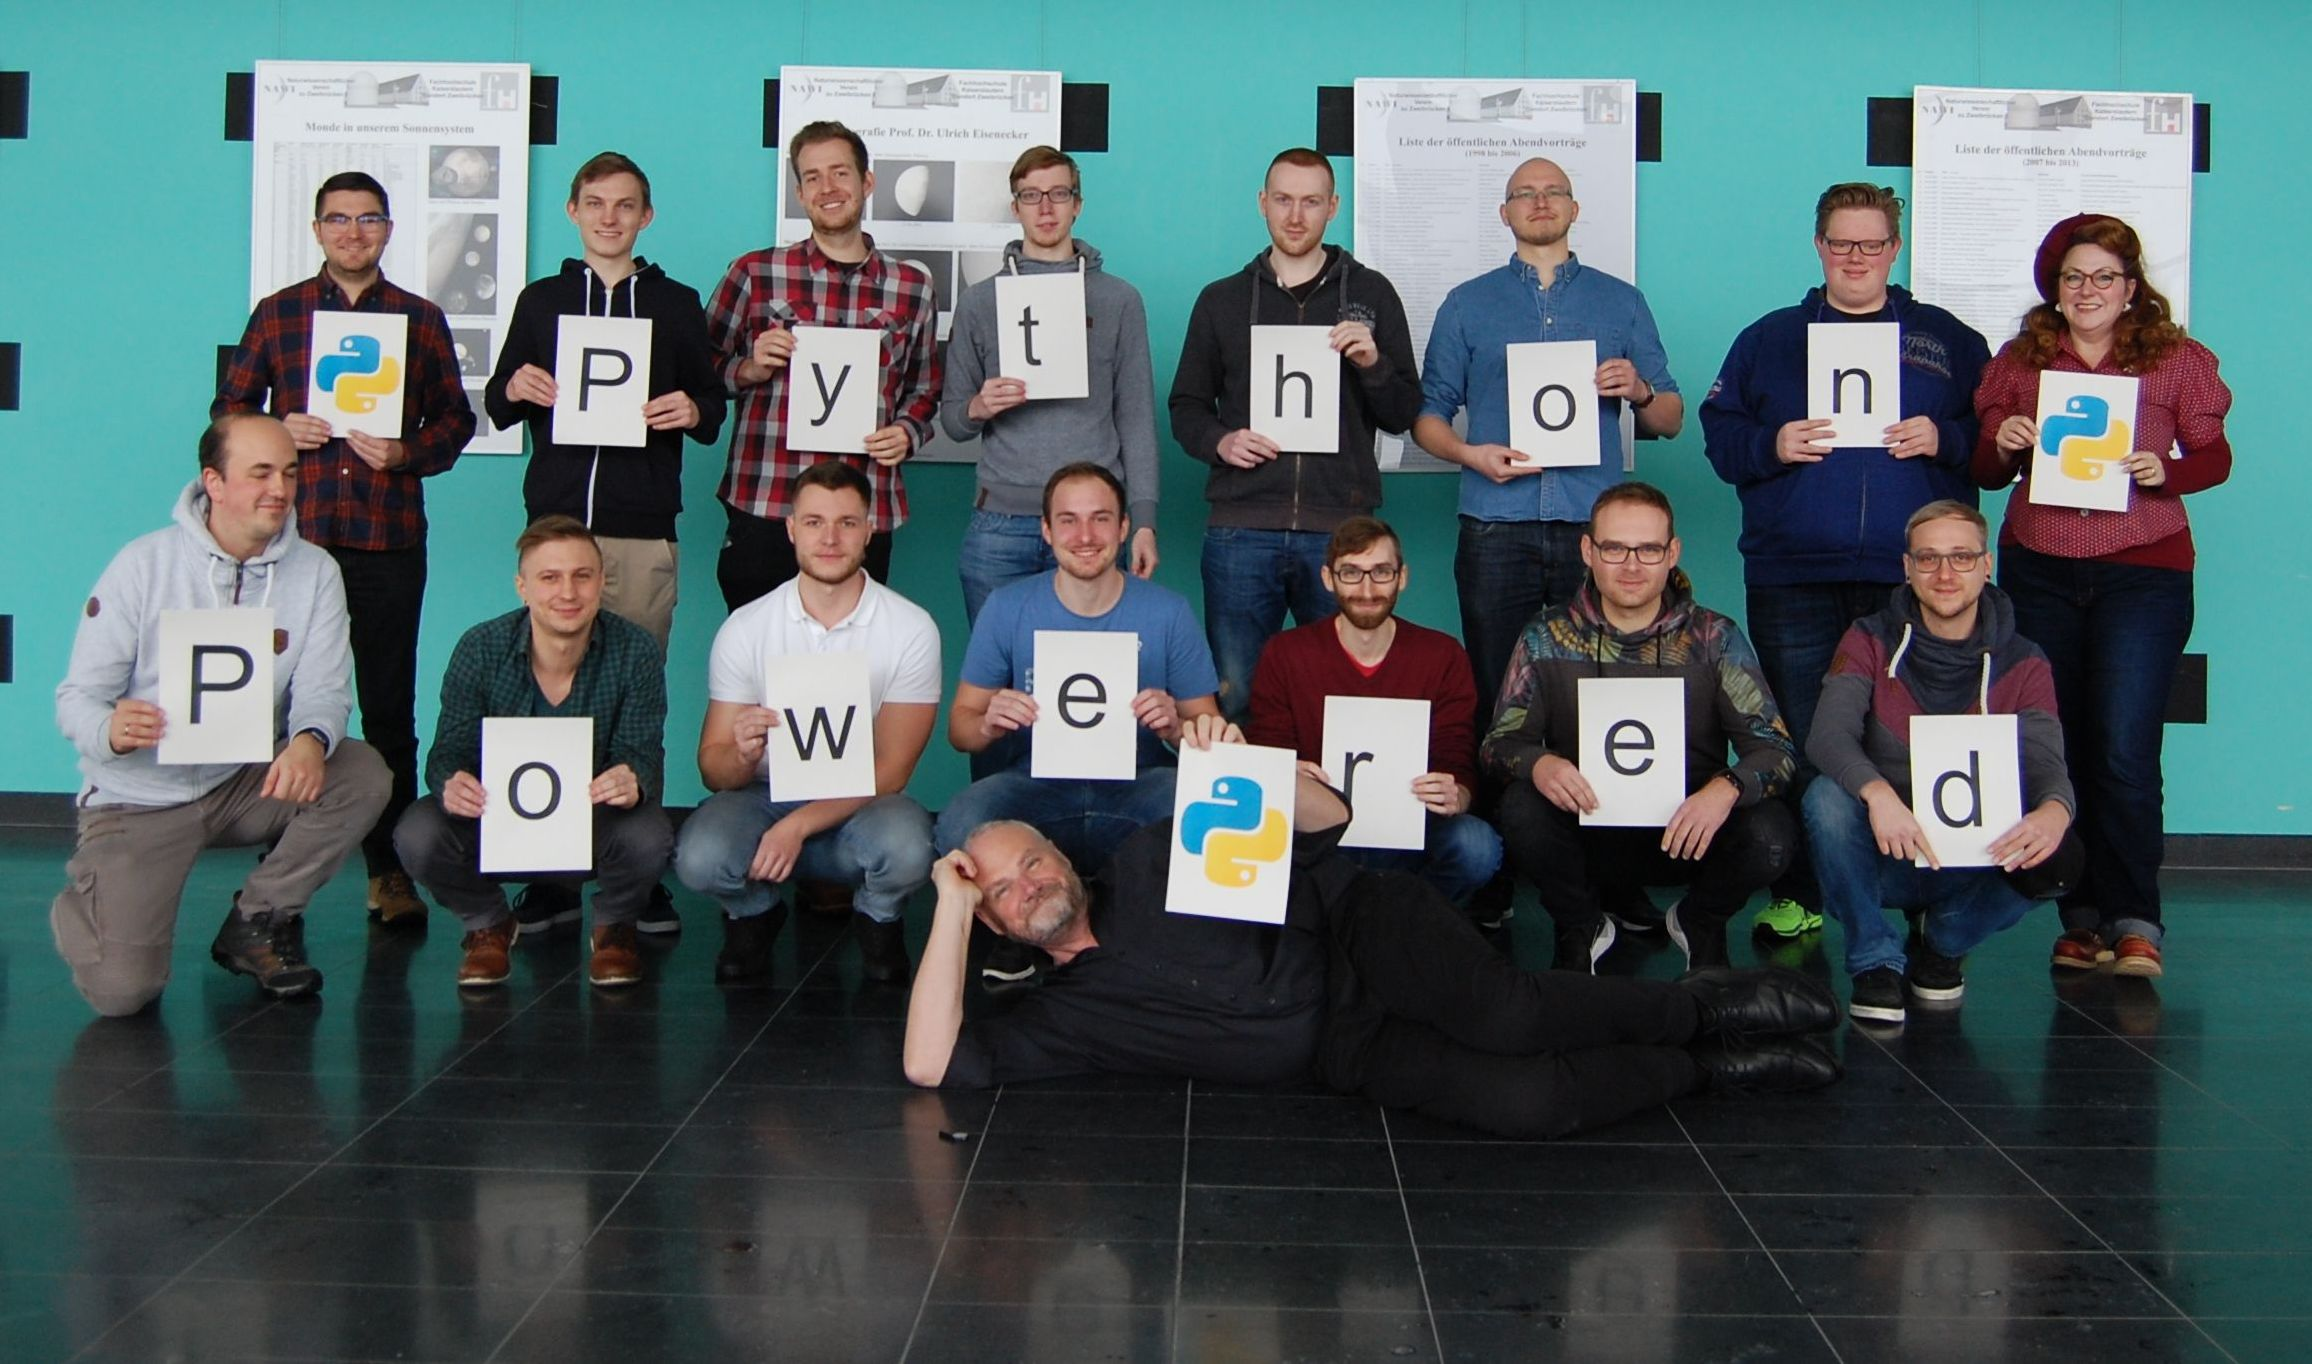
\includegraphics[width=\textwidth]{images/authors/theTeam}% Rotieren mit rotate=90
%\caption{\label{vorwort:team}Das Projektteam}
\end{figure}
\begin{tabular}{ll}
\centering
&Das Projektteam nach dem letzten Sprint Meeting\\
& im Januar 2019 von links nach rechts:\\
Hintere Reihe&Fabian Kalweit, Matthias Haselmaier, Marc Zintel,\\
                   &Robin Guth, Anatoli Sch�fer, Denis Schlusche,\\
                   &Kevin Konrad, Miriam Lohm�ller \\
Vordere Reihe&Mathias Fedder, Rainer Haffner, Lukas Kuhn,\\
                   &Sebastian Morsch, Julian Bernhart, Phillip Lauer,\\
                   &Christoph Seibel\\
Ganz vorne&Manfred Brill
\end{tabular}

\pagebreak
\subsection*{Die studentischen Autoren}
\begin{center}
\begin{tabular}{p{5cm}|l}
Julian  Bernhart&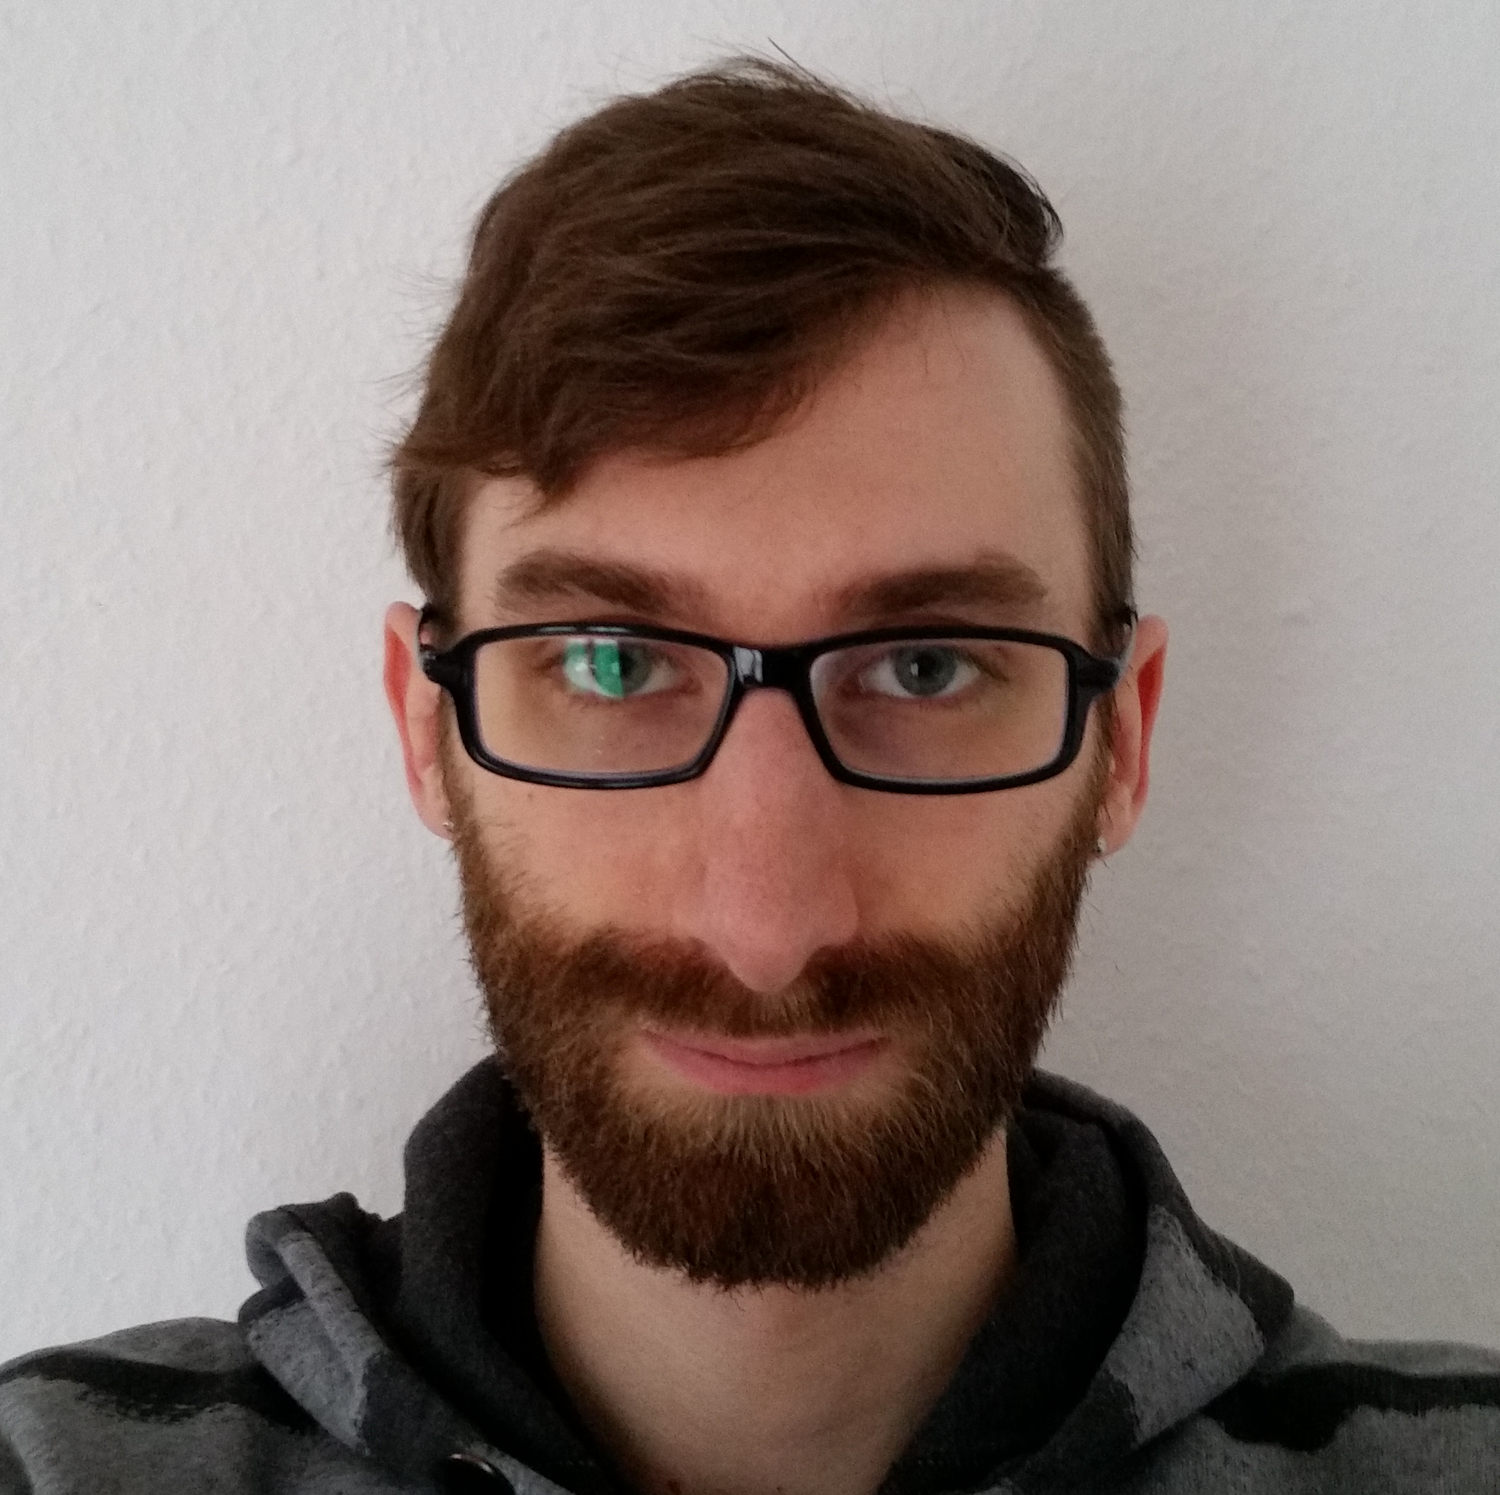
\includegraphics[width=3cm]{images/authors/bernhart}\\
Eric Brunk&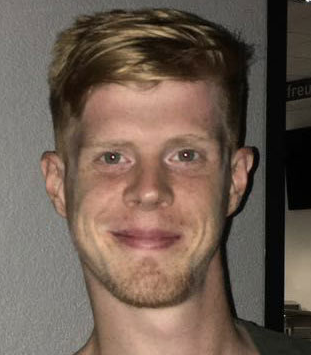
\includegraphics[width=3cm]{images/authors/brunk}\\
Mathias Fedder&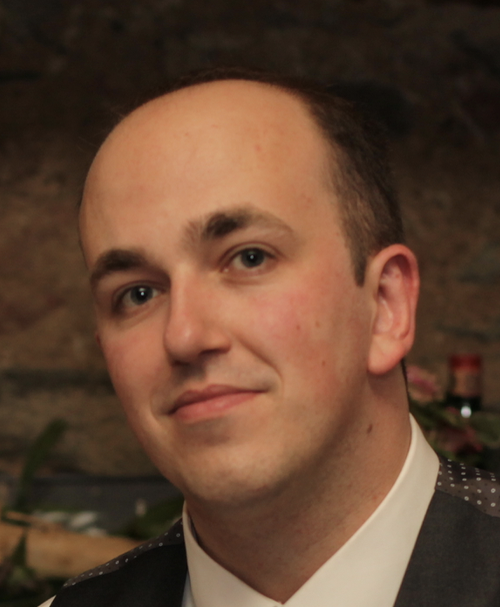
\includegraphics[width=3cm]{images/authors/fedder}\\
Christopher Gross&\\
Robin Guth&\\
Rainer Haffner&
\includegraphics[width=3cm]{images/authors/haffner}\\
Matthias Haselmaier&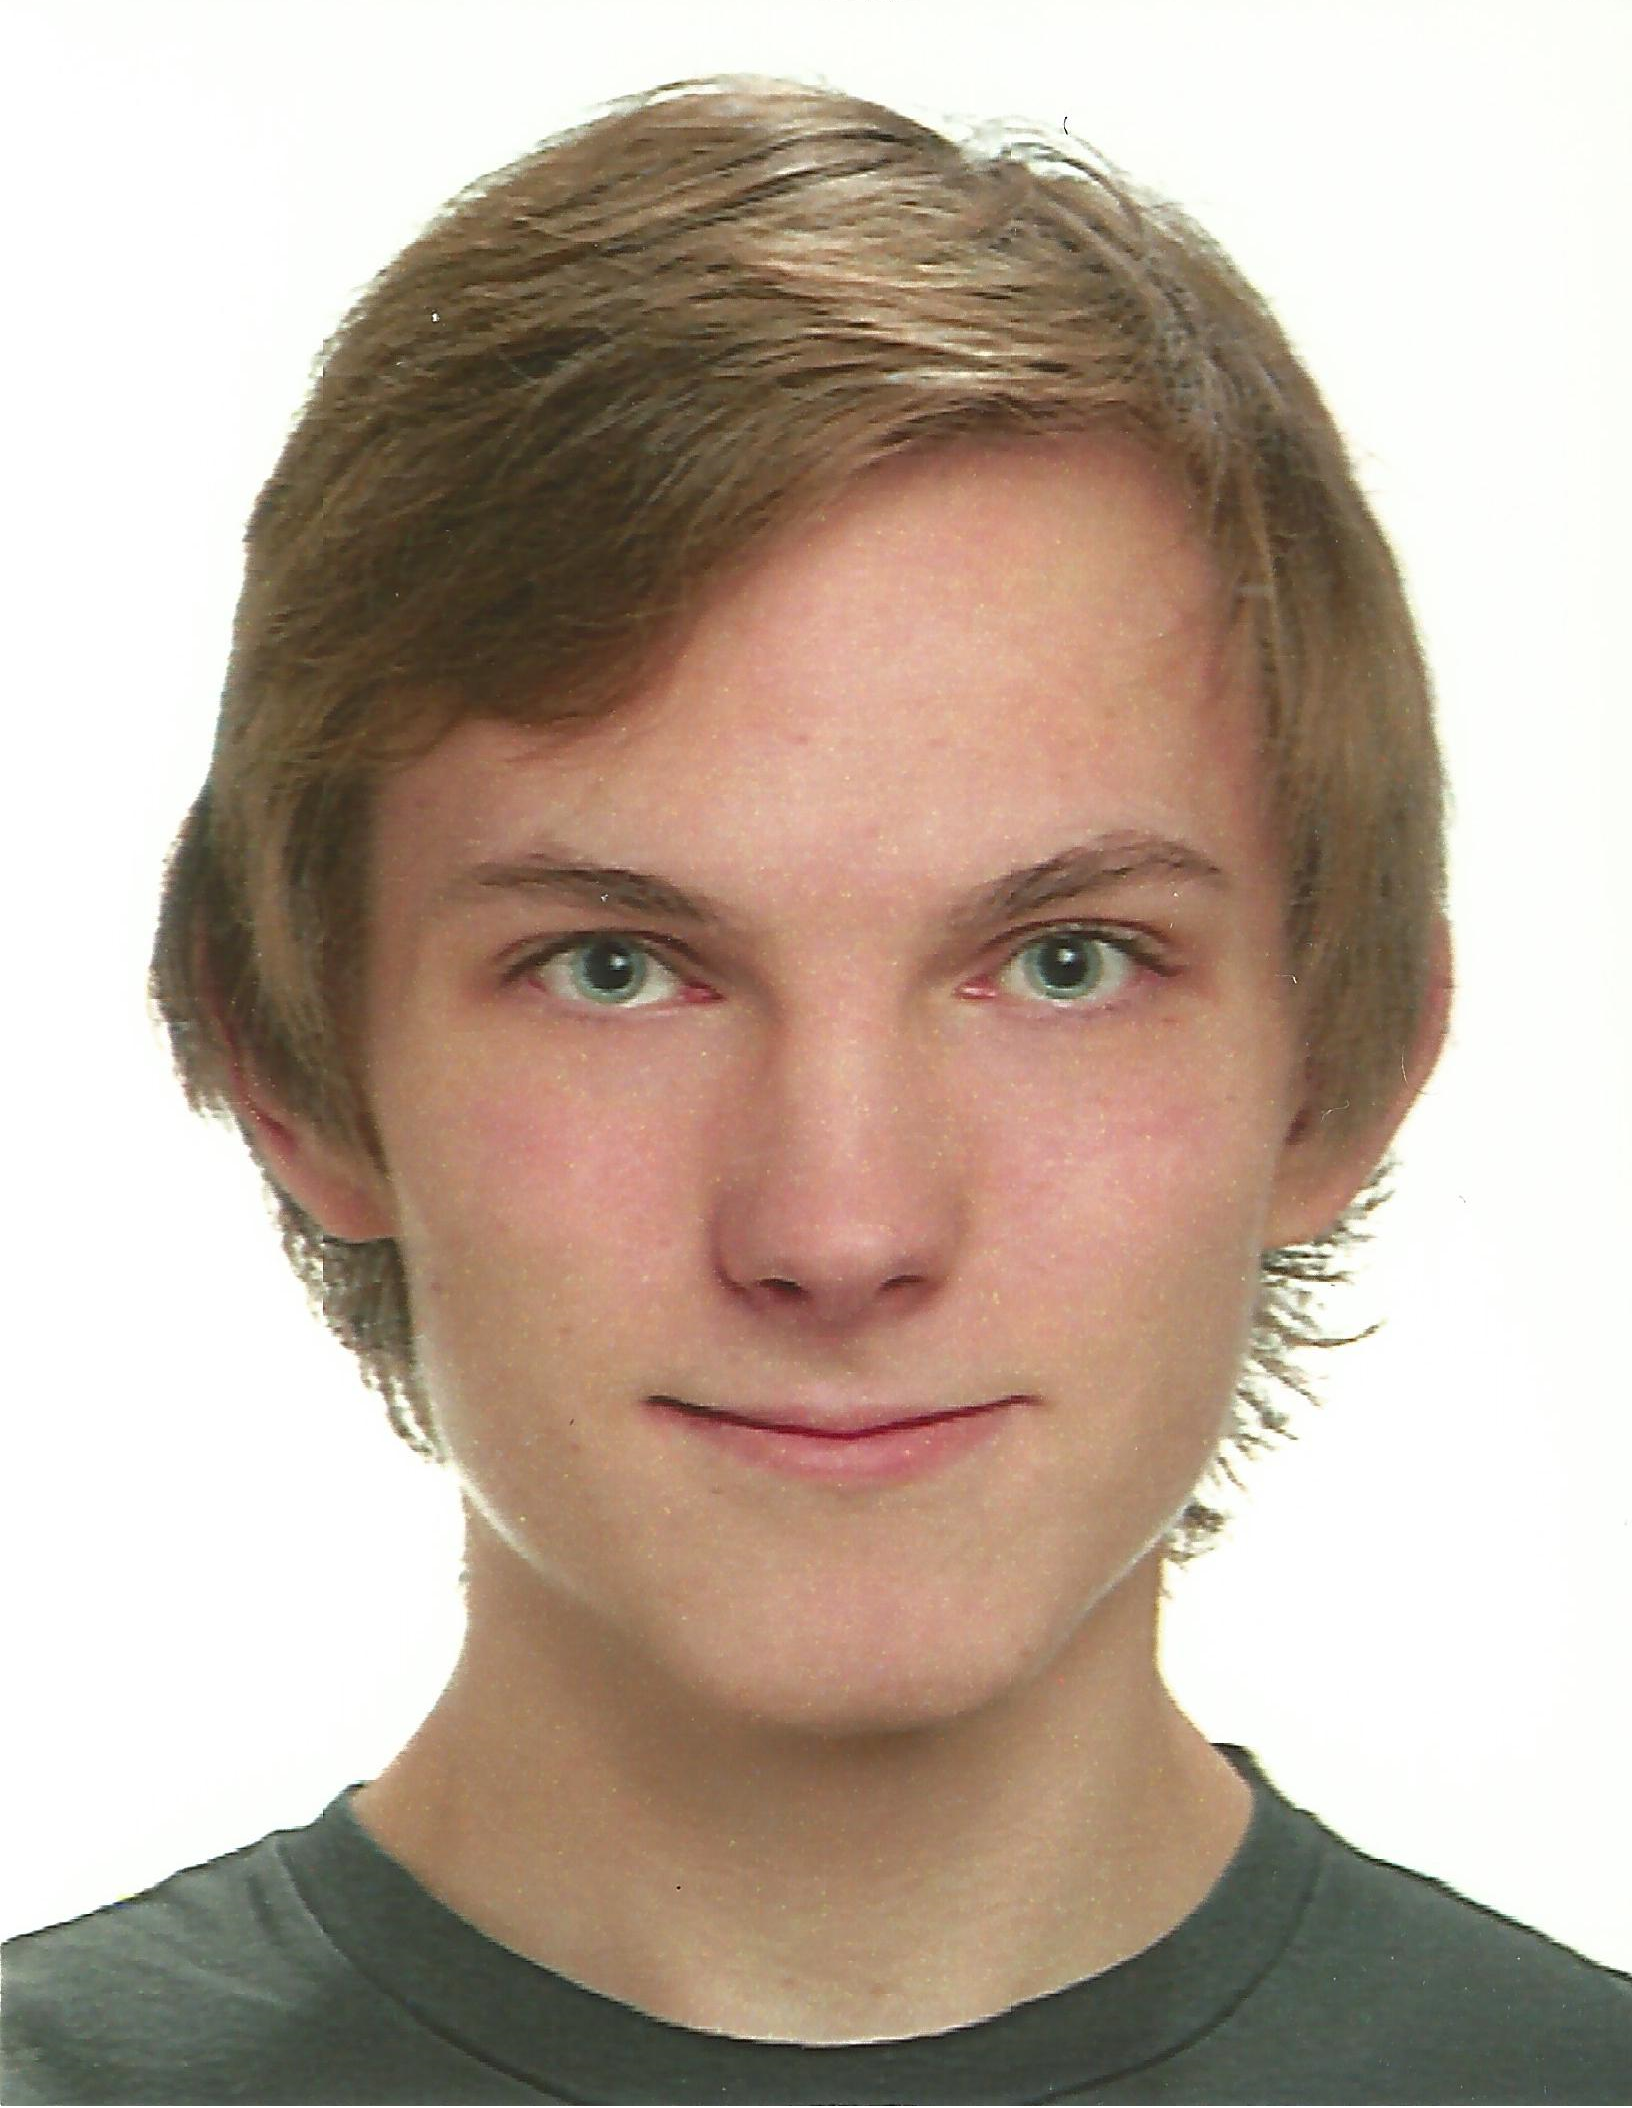
\includegraphics[width=3cm]{images/authors/haselmaier}\\
Kevin Konrad&\\
Lukas Kuhn&
\end{tabular}
\end{center}
\pagebreak
\begin{center}
\begin{tabular}{p{5cm}|l}
Philipp Lauer&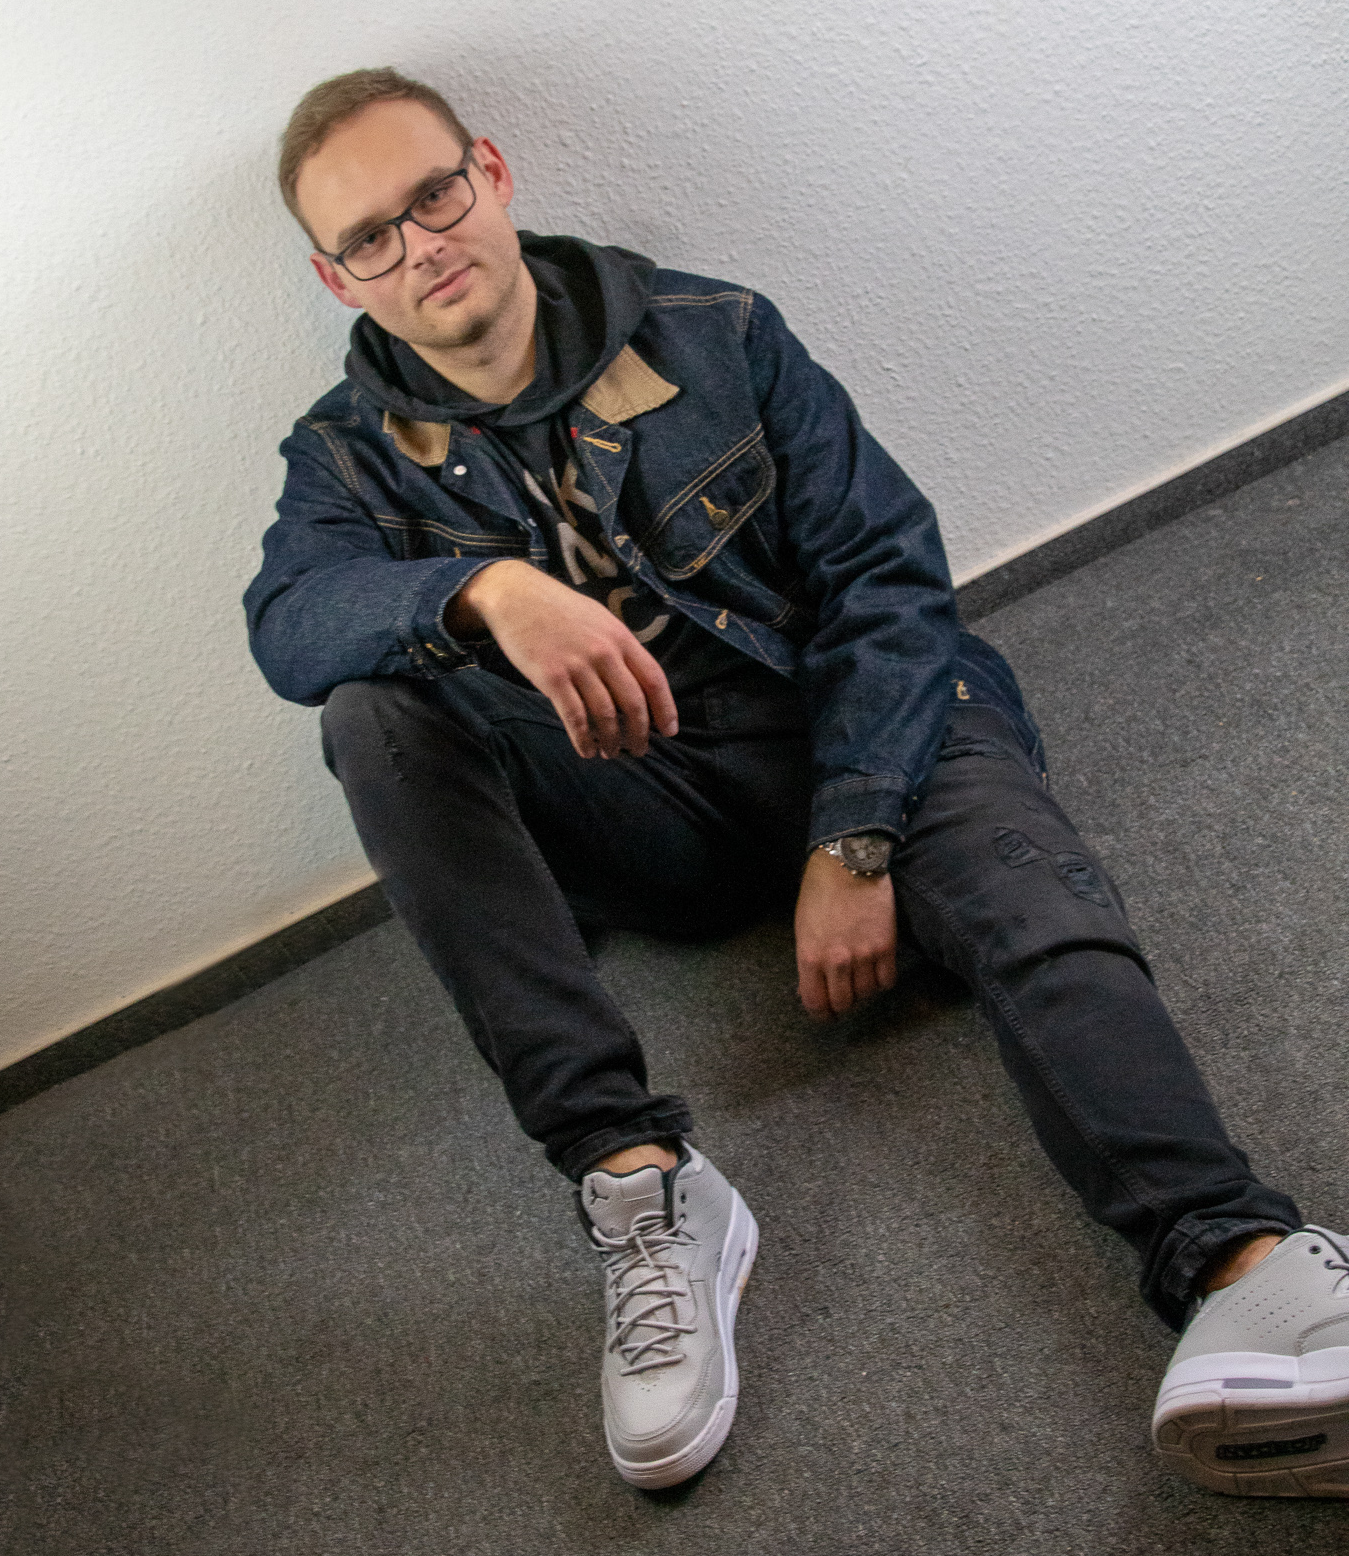
\includegraphics[width=3cm]{images/authors/lauer}\\
Sebastian Morsch&\\
Anatoli Sch�fer&\\
Denis Schlusche&\\
Christoph Seibel&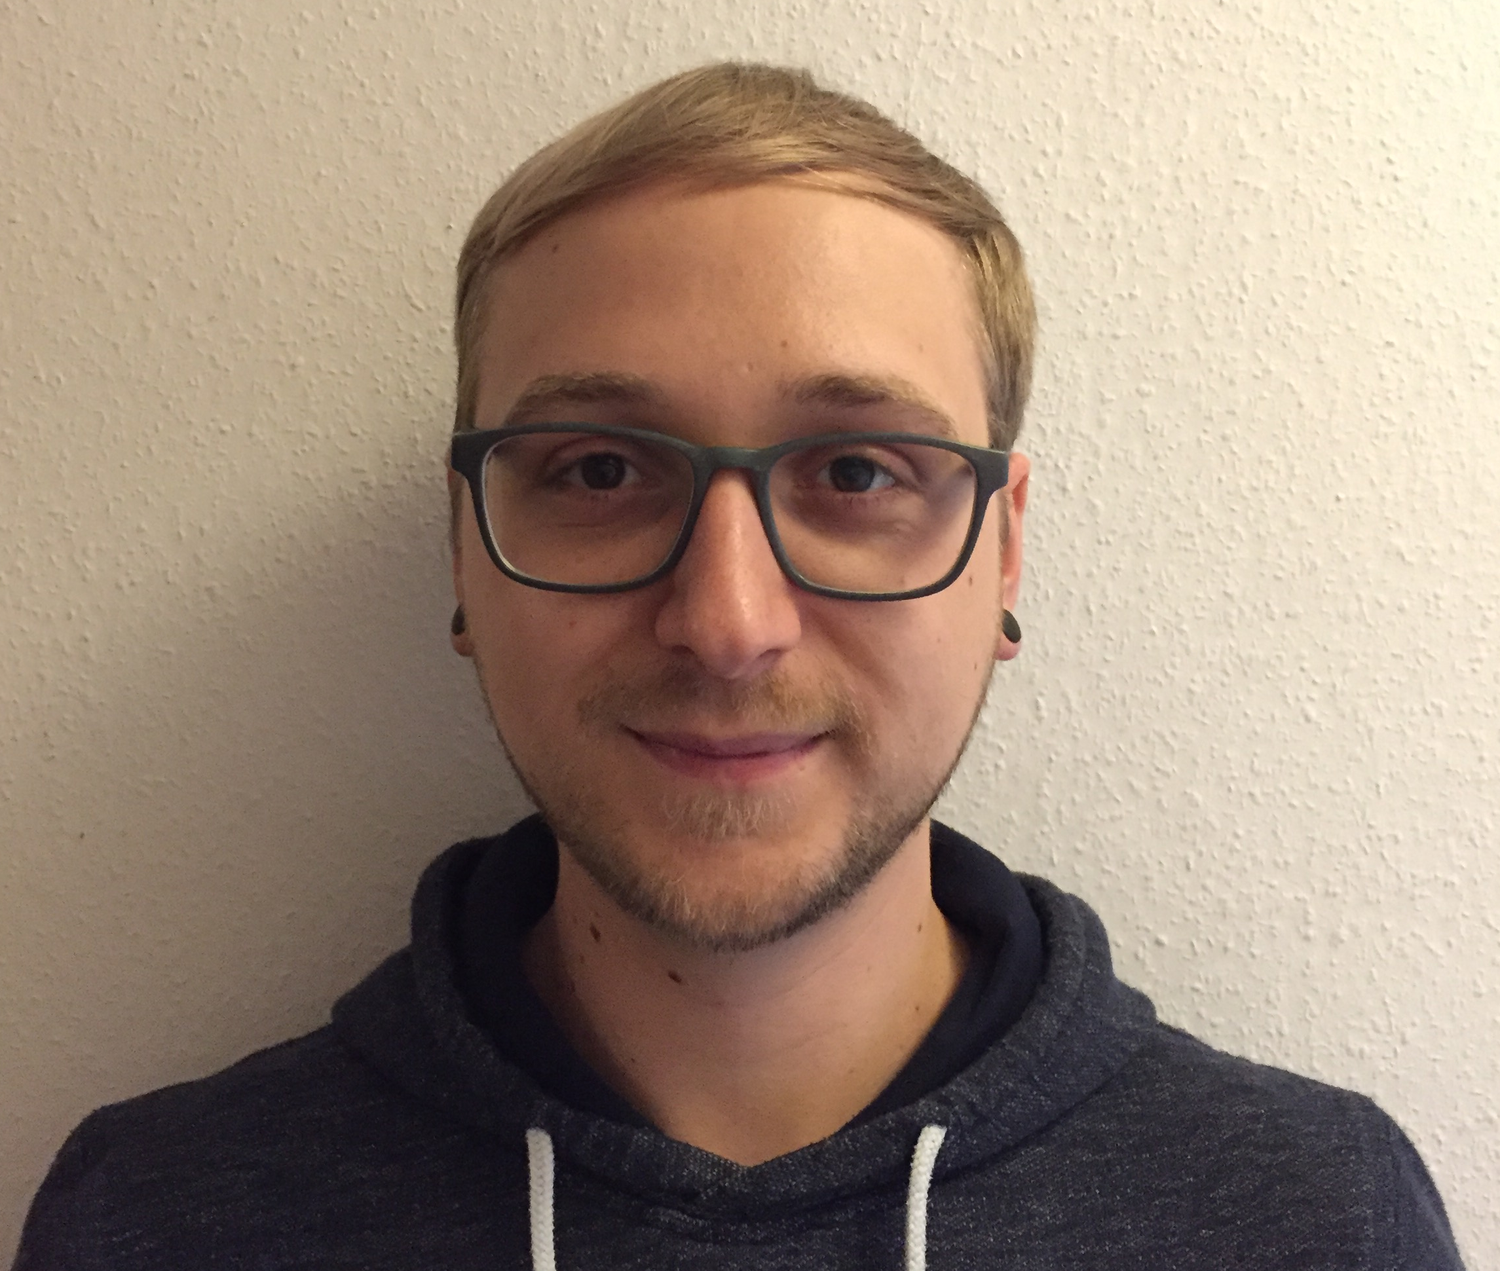
\includegraphics[width=3cm]{images/authors/seibel}\\
Marc Zintel&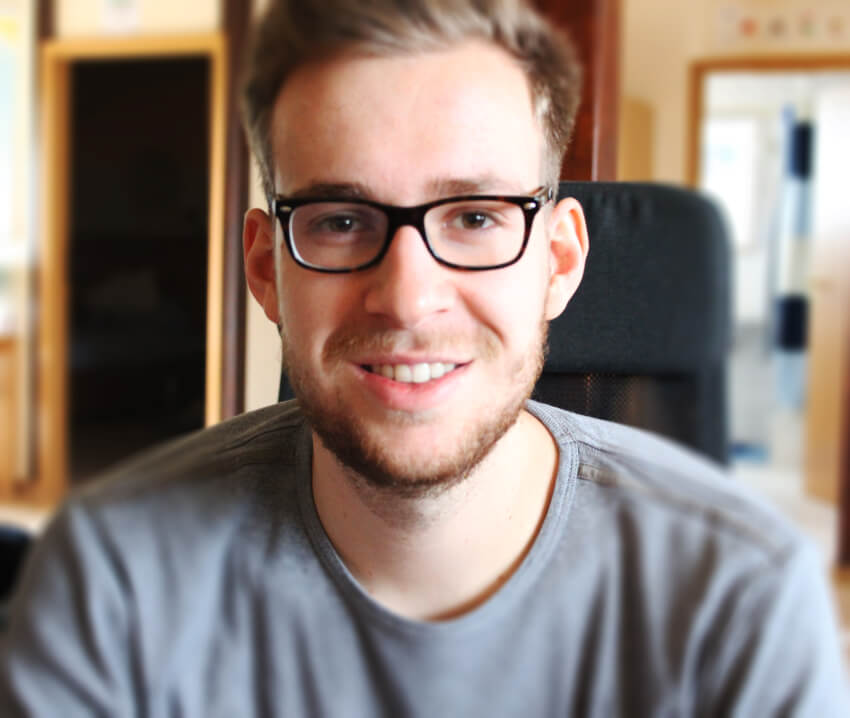
\includegraphics[width=3cm]{images/authors/zintel}
\end{tabular}
\end{center} 
%
% Inhaltsverzeichnis
%
\tableofcontents
\clearevenpage
\pagenumbering{arabic}
%
%
%

% !TeX root = ../pythonTutorial.tex
\chapter{Idee}

Der Grundgedanke hinter dem Virtual Science Lab ist es, Wissenschaft m�glichst anschaulich und spielerisch zu vermitteln. Dabei kommen die technischen Mittel der Virtual Reality zum Einsatz. Diese soll sicherstellen, dass die Versuche m�glichst nativ durchgef�hrt werden k�nnen, das hei�t dass beispielsweise Gegenst�nde durch Hinf�hren der Hand und anschlie�endes Zugreifen eines Buttons aufgehoben werden k�nnen. Auch ein normales Bewegen im Raum ist m�glich, weshalb die Annahme besteht, dass die Einstiegsh�rde deutlich geringer ist, als beispielsweise eine Steuerung mit Maus und Tastatur oder Gamepad. Auch der visuelle Eindruck soll durch den Einsatz von Virtual Reality gesteigert werden, da man sich frei im Raum drehen und bewegen kann und so zur Erkundung angeregt wird. Das Virtual Science Lab wird zun�chst auf der HTC Vive Pro entwickelt und evaluiert.


\begin{figure}
	\centering
	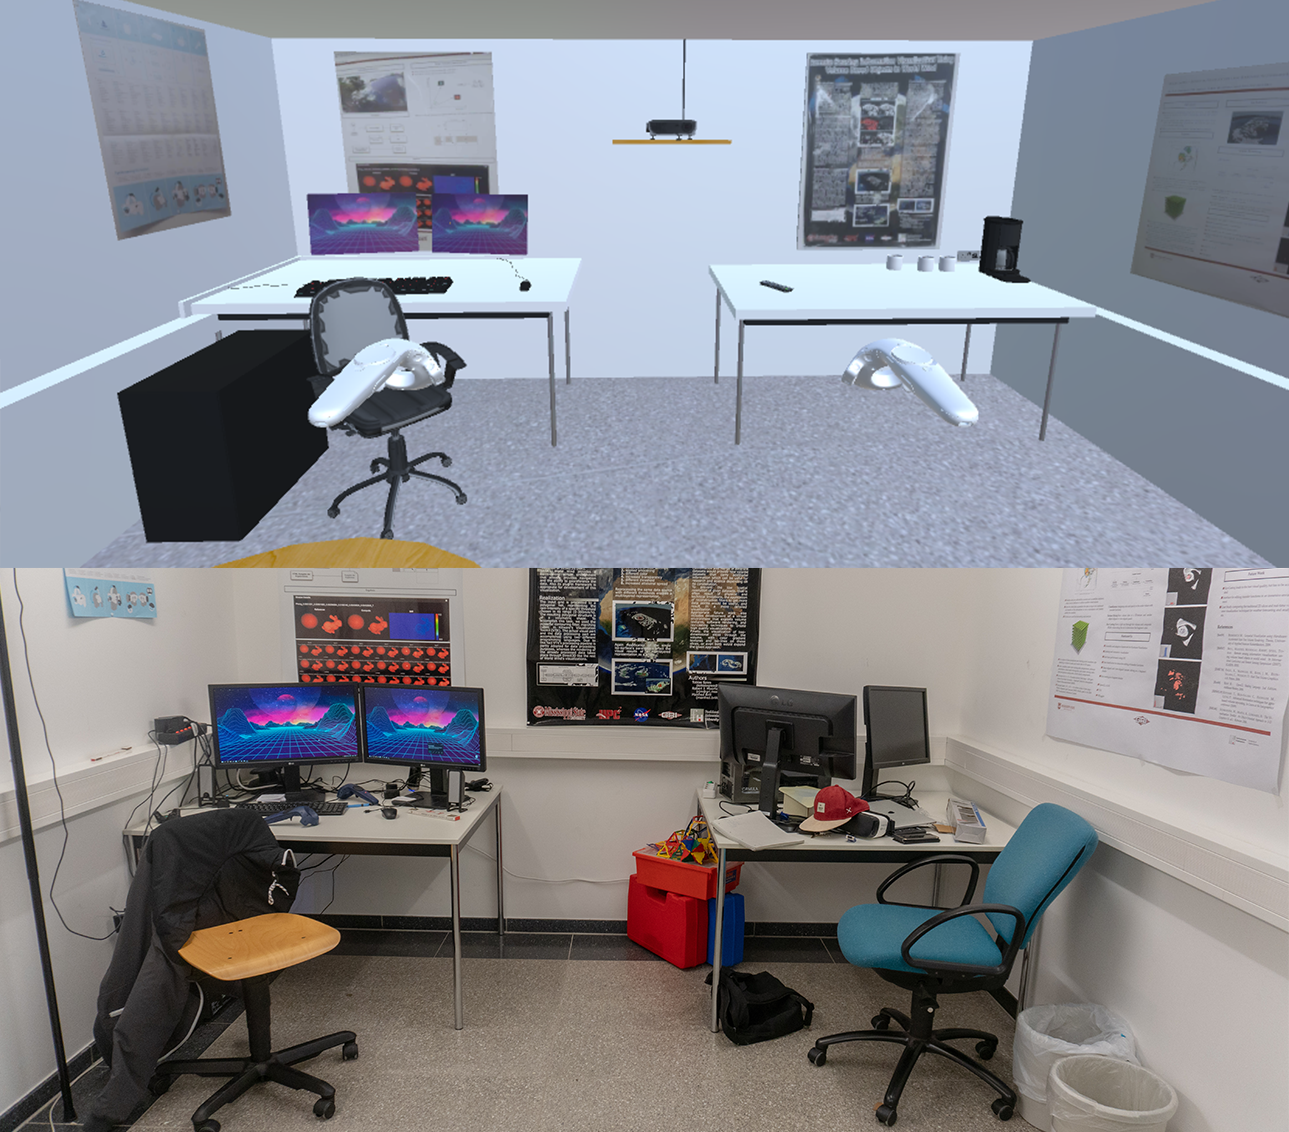
\includegraphics[width=1\textwidth]{images/labor/labor_vgl.png}
	\caption{Vergleich reales Labor - virtuelles Labor}
	\label{img:labor}
\end{figure}
% !TeX root = ../pythonTutorial.tex
\chapter{Steuerung}

Gesteuert wird die gesamte Anwendung mit den Controllern der HTC Vive Pro. Au�erdem wird durch Sensoren im VR-Labor erm�glicht, sich innerhalb des Raumes von drei auf vier Metern (bis zu zehn auf zehn Meter m�glich) frei im Raum zu bewegen. Verwendet man die wireless Variante, erm�glicht dies ein sehr freies und angenehmes Erlebnis. Da man in der virtuellen Realit�t schnell den �berblick verlieren kann, wie weit die jeweiligen W�nde des Raumes noch in Wirklichkeit entfernt sind, wird ein Gitter in der Anwendung angezeigt, wenn man sich dieser zu sehr n�hert. 

Da einer der R�ume f�r die potenzielle Nutzung der maximal m�glichen Raumgr��e entworfen wurde, ist eine Teleport-M�glichkeit unerl�sslich. Diese ist jedoch auch im Flur n�tig und in den anderen R�umen m�glich. Durch Dr�cken des Touchpads des Controllers erscheint ein Marker, den man auf die am Boden befindliche Stelle platzieren muss, an die teleportiert werden soll. Durch Loslassen wird man zur gew�nschten Stelle gebracht.
Die einzige andere Taste, die zur Bedienung verwendet wird, ist der Hairtrigger. Mit diesem lassen sich Gegenst�nde durch Ber�hrung und gleichzeitiges gedr�ckt Haltens des Triggers hochheben. Ein Teleport mit einem aufgehobenen Gegenstand im selben Controller ist nicht m�glich, dazu sind beide Controller notwendig. Mit einem muss man den Gegenstand mit dem Hairtrigger aufnehmen und halten, mit dem anderen wird �ber das Touchpad teleportiert.

% !TeX root = ../pythonTutorial.tex
\chapter{Bisheriger Stand}

Die Ausgangslage zu Projektstart, bildete die Vorarbeit im Fach ?Augmented und Virtual Reality?, bei dem das Virtual Science Lab zusammen noch mit Anatoli Sch�fer erste Z�ge angenommen hat. In diesem Kontext wurden 4 Laborr�ume kreiert, sowie eine Outdoor Area, die lediglich zur Erkundung im virtuellen Raum dienen sollte. 
Als Startpunkt des Projektes diente ein Nachbau des Virtual Reality Labor der Hochschule Kaiserslautern, Standort Zweibr�cken. Da das Projekt voraussichtlich dort durchgef�hrt werden sollte, zieht der User die Brille an und befindet sich danach im gleichen Raum, in dem er ohne Brille gestanden hat ? nur eben virtuell. 
Des Weiteren bekam das Projekt ein Chemielabor, sowie zwei Laborr�ume mit Versuchen die eine Mischung zwischen Physik und Chemie zeigen. Diese waren ein Versuch zur Flammenf�rbung, ein Leitbarkeitstest und eine Reaktion zwischen zwei Stoffen (M�llverarbeitung). Die letzten beiden R�ume wurden durch einen gewinkelten Gang miteinander verbunden, der lediglich dem Zweck dienen sollte. In allen R�umen sind Erkl�rungen zu den Versuchen in verschiedener Form platziert (Klemmbrett, Beamer, Plakate).


\clearpage
\begin{figure}
	\centering
	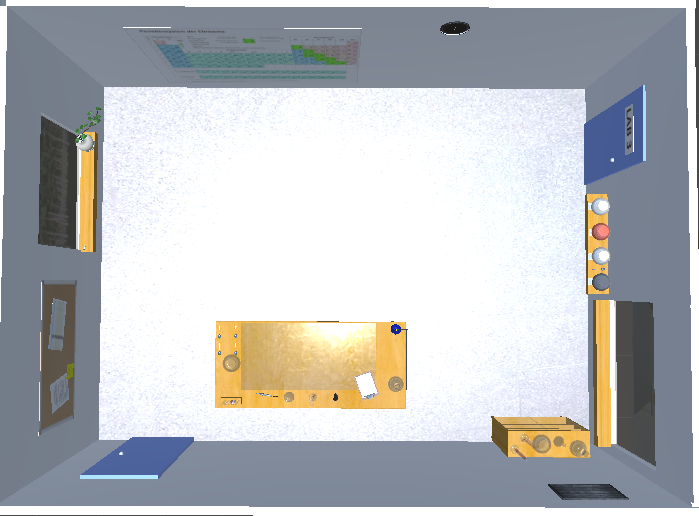
\includegraphics[width=1\textwidth]{images/bisheriger_stand/grundriss_chemielabor.png}
	\caption{Grundriss Chemielabor}
	\label{img:chemielabor}
\end{figure}
\begin{description}
	\item[Flammenf�rbung:]\hfill \\
	Im Raum befinden sich verschiedene L�ffel, ein Bunsenbrenner (auf Grund fehlender Modelle ein Zylinder mit Knopf) und verschiedene Stoffe auf einer Ablage (Calcium, Kalium, Lithium und Kupfer). Man nimmt einen L�ffel, nimmt einen beliebigen Stoff auf, schaltet den Bunsenbrenner an und h�lt den L�ffel in die Flamme. Anschlie�end betrachtet man die gef�rbte Flamme
\end{description}
\begin{description}
	\item[M�llverarbeitung:]\hfill \\
	Der Raum ist angef�llt mit K�rpern aus Styropor. In der Mitte des Raumes befindet sich ein Tisch mit einer Schale voll Aceton. Nimmt man die Styropork�rper auf und wirft sie in die Schale l�sen sie sich nach einiger Zeit auf.
\end{description}
\begin{description}
	\item[Leitbarkeitstest:]\hfill \\
	Auf einem Tisch befindet sich ein Beh�ltnis mit Wasser. Durch das Gef�� l�uft ein Draht der einen Lichtschalter und eine Gl�hbirne verbindet. Da destilliertes Wasser keinen Strom leitet bewirkt das Tasten des Schalters im Ausgangszustand nichts. Erst muss ein leitbarer Stoff, in diesem Fall Salz dem Wasser hinzugegeben werden. Anschlie�end l�sst sich die Lampe einschalten.
\end{description}

Das Git-Repository (vgl. \cite{VSL}) des bestehenden Projektes wurde fortgesetzt. Dort l�sst sich neben der aktuellsten Version auch der Ausgangsstand vor Projektbeginn herunterladen. Dieses ist die Version 1.0 vom 15. August 2019, zu finden im Projekt unter Releases.
% !TeX root = ../pythonTutorial.tex
\chapter{Neuerungen}

Da bereits erste Erfahrungen mit Unity gemacht werden konnten, wurden zu Beginn des Projektes die Ziele h�hergesteckt als bei der bisherigen Ausf�hrung. Neben vielen Wissenschaftszweigen wie Mathematik, Informatik, Biologie etc. sollte auch ein Android Build erstellt werden, der auf preiswerten Ger�ten ausgerollt werden sollte. Die Idee dahinter ist es, dass in einem Klassenraum jeder f�r sich einen Versuch selber durchf�hren soll, statt lediglich aus mehreren Metern entfernt zuzuschauen, wie der Lehrer den Versuch zum zigsten Mal in seiner Laufbahn macht. \newline
Au�erdem sollte der bisherige Aufbau insgesamt etwas abge�ndert werden, sowie bestehende Bugs behoben werden. Ideen kamen viele, meist bestand das Problem in der bildlichen Vorstellung. Wie soll ein theoretischer Versuch m�glichst anschaulich in VR umgesetzt werden und anschlie�end sinnvoll und nativ durchf�hrbar sein. Die Outdoor Area wurde komplett entfernt, ebenso wie der gewinkelte Gang zwischen dem Leitbarkeitstest und der M�llverarbeitung. 

\begin{figure}
	\centering
	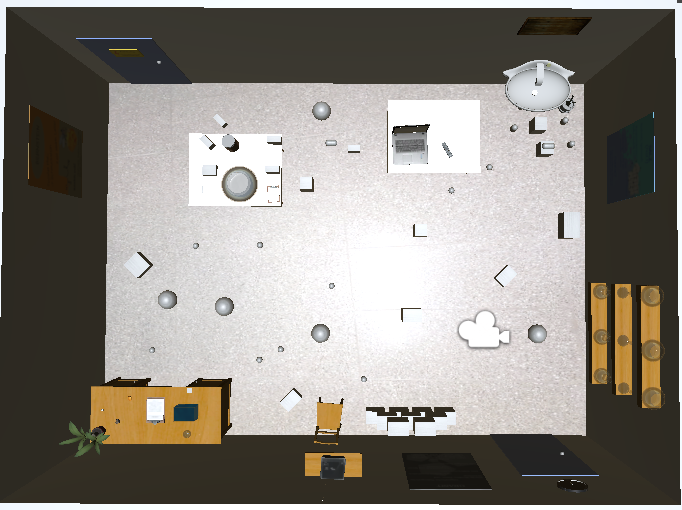
\includegraphics[width=1\textwidth]{images/neuerungen/grundriss_physiklabor.png}
	\caption{Grundriss Physiklabor}
	\label{img:physiklabor}
\end{figure}

Die ganzen Labore sollten durch einen einzelnen breiten Flur mit T�ren zu jedem Versuch zug�nglich werden. Leitbarkeitstest und M�llverarbeitung wurden zus�tzlich zusammengelegt unter dem Oberbegriff \textit{Physik}. Das Chemielabor hat ein richtiges Bunsenbrenner-Modell erhalten. Das VR- Lab, das vorher keinen eigenen Versuch erhalten hatte, bekam nun einen eigenen Versuch, beziehungsweise eher ein bekanntes Knobelspiel: \textit{Die T�rme von Hanoi} in Lebensgr��e. Die neu gefertigten R�ume mit den dazugeh�rigen Versuchen werden im Folgenden mit den aufgetretenen Problemen veranschaulicht:

\begin{figure}
	\centering
	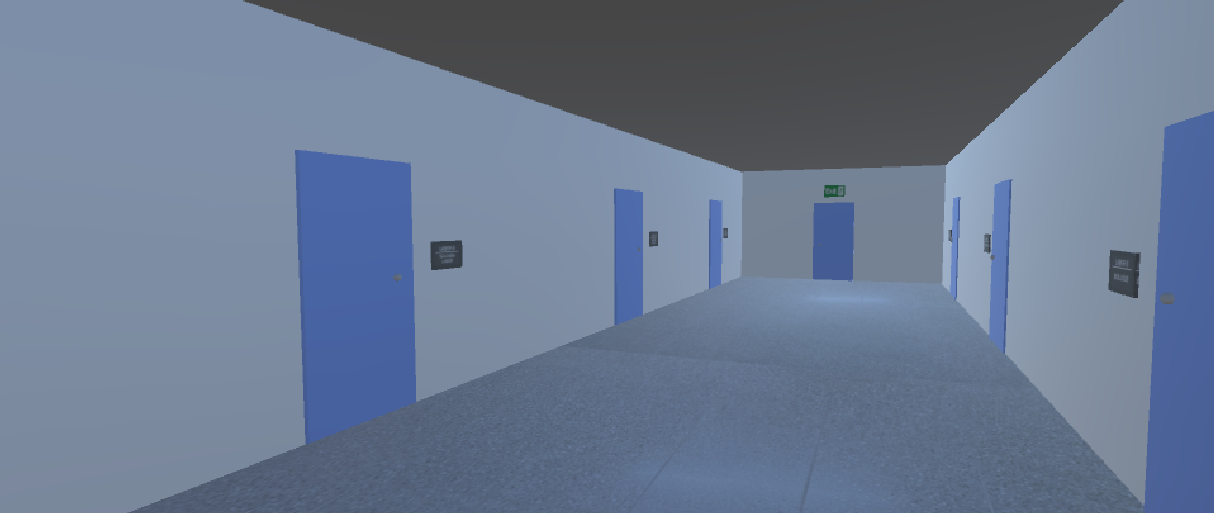
\includegraphics[width=1\textwidth]{images/neuerungen/neuer_flur.png}
	\caption{Neuer Flur mit T�ren zum jeweiligen Laborraum}
	\label{img:neuerflur}
\end{figure} 
\begin{figure}
	\centering
	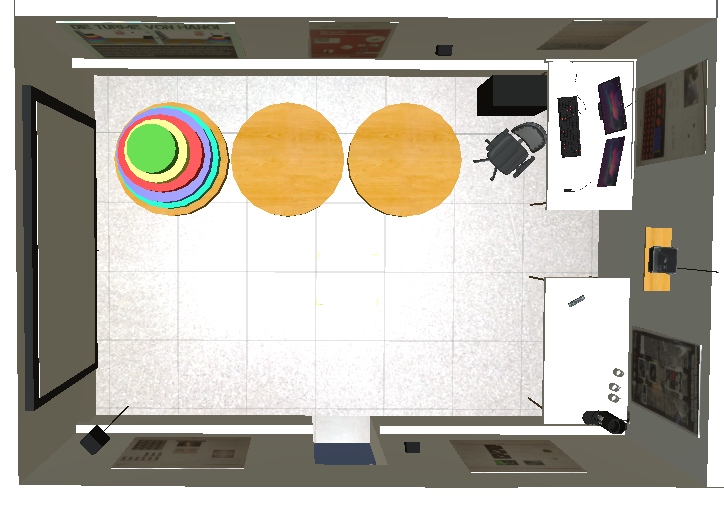
\includegraphics[width=1\textwidth]{images/neuerungen/grundriss_vrlab.png}
	\caption{Grundriss Virtual Reality Labor}
	\label{img:vrlab}
\end{figure}


\section{Biologie}

Das Biologie Labor hat einen Mikroskop-Versuch. Auf einem Tisch im Raum liegen drei Glasplatten mit verschiedenen Inhalten (Blut, Pflanze, Textil). Diese Platten kann man aufnehmen und in das Mikroskop [2], das auf dem danebenstehenden Tisch (soll zur Bewegung im Raum animieren) steht einlegen. Klickt man nun erneut auf das Mikroskop gelangt man in das zu betrachtende Material. Durch eine Fallt�r auf dem Boden kann man wieder zur�ck ins Labor gelangen. Die Fallt�r soll dazu dienen, dass man auch die H�he des Raumes mit einbezieht und der User gezwungen ist, sich zu b�cken. 

\begin{figure}
	\centering
	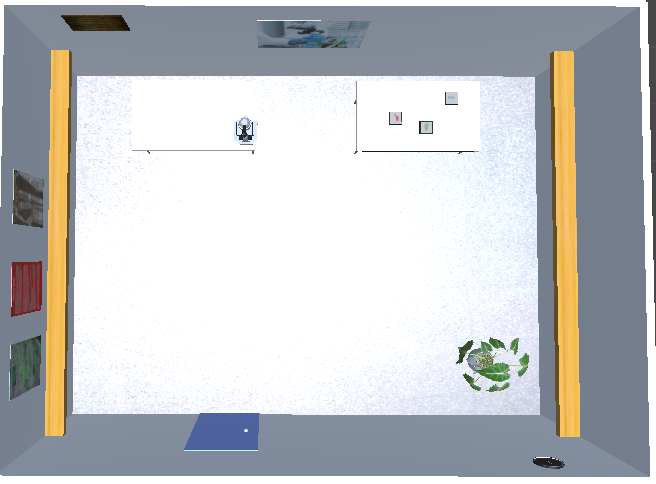
\includegraphics[width=1\textwidth]{images/neuerungen/grundriss_biolab.png}
	\caption{Grundriss Biologielabor}
	\label{img:biolab}
\end{figure}
\begin{figure}
	\centering
	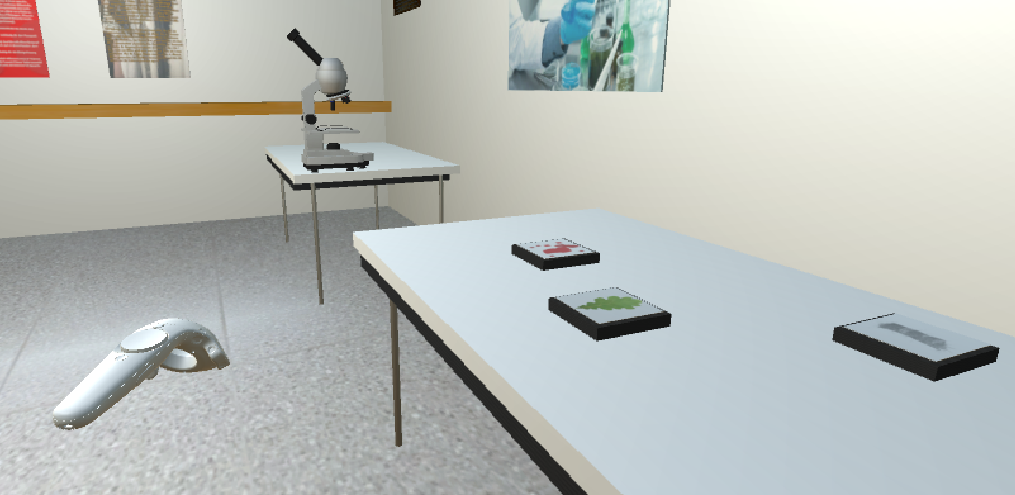
\includegraphics[width=1\textwidth]{images/neuerungen/biolab_mikroskop.png}
	\caption{Biologielabor mit Mikroskop und Glasplatten}
	\label{img:biolabmikroskop}
\end{figure}
\begin{figure}
	\centering
	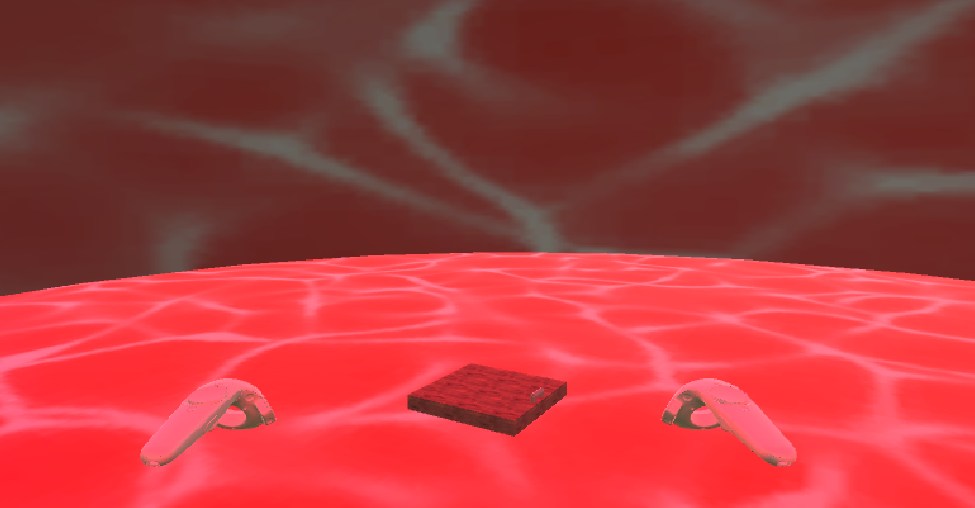
\includegraphics[width=1\textwidth]{images/neuerungen/biolab_blutzelle.png}
	\caption{Biologielabor Blutzelle}
	\label{img:biolabblutzelle}
\end{figure}
\begin{figure}
	\centering
	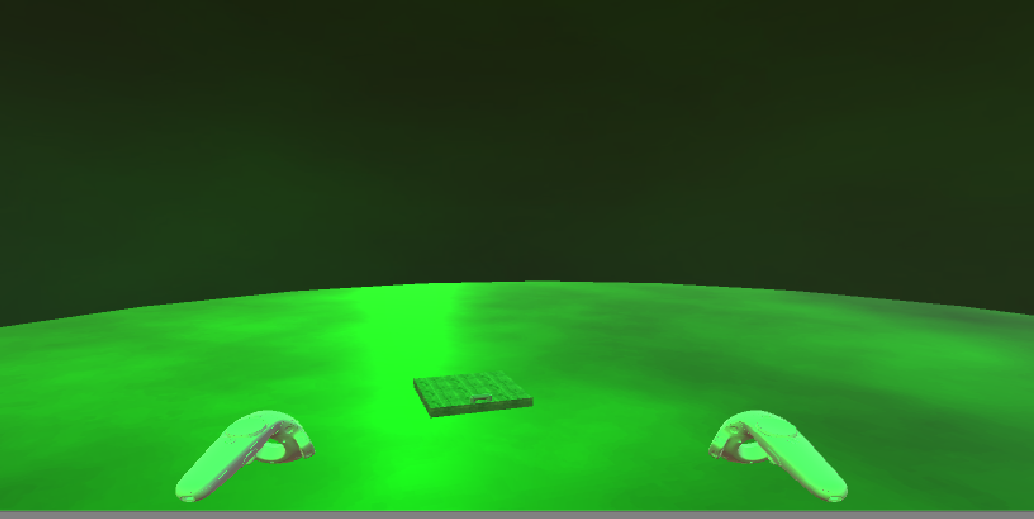
\includegraphics[width=1\textwidth]{images/neuerungen/biolab_pflanze.png}
	\caption{Biologielabor Pflanzenzelle}
	\label{img:biolabpflanze}
\end{figure}
\begin{figure}
	\centering
	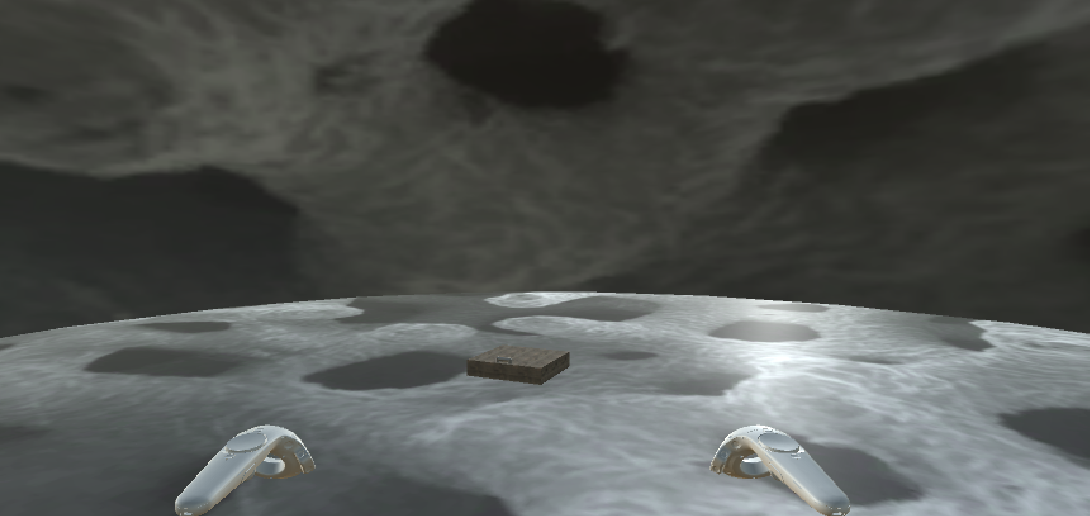
\includegraphics[width=1\textwidth]{images/neuerungen/biolab_textil.png}
	\caption{Biologielabor Textilfaser}
	\label{img:biolabtextil}
\end{figure}

In diesem Labor bestand ein Problem darin, die Szenen f�r Pflanze, Blut und Textil zu gestalten, da Unity nicht von sich aus eine Sphere von innen texturiert. Das hei�t, wenn man eine gro�e Sphere als Art Kuppel anlegen will, funktioniert dies nicht einfach, indem man die Kamera innerhalb der Sphere platziert. Nach einer Recherche mit einigen Umwegen war die L�sung sehr simpel, es wurde ein Double Side Shader statt dem Standard Shader ausgew�hlt, sowie die Belichtung angepasst. 

\clearpage
\section{Mathematik}

Ein Raum des Projektes sollte planm��ig die bisherigen Ma�e von 3x4 Meter durch 10x10 Meter ersetzen, sodass auch Vorf�hrungen in einem gr��eren Raum sinnvoll sind.  Dabei fiel die Wahl auf das Mathematiklabor. In diesem wurde die Darstellung der Kardioiden-Funktion aus der Outdoor Szene recyclet, welche man nun mit der dazugeh�rigen Gleichung durch ein Fenster au�erhalb des Raumes betrachten kann.  \newline

Au�erdem wurde das K�nigsberger Br�ckenproblem raumf�llend gestaltet. Dem Benutzer ist es also m�glich, sich frei innerhalb des Raumes zu bewegen, um zu versuchen das nicht l�sbare Problem zu l�sen. Die L�sung ist etwas versteckt in Form eines ''toten Briefkastens'', der sich unter ein paar Steinen befindet. \clearpage 

\begin{figure}
	\centering
	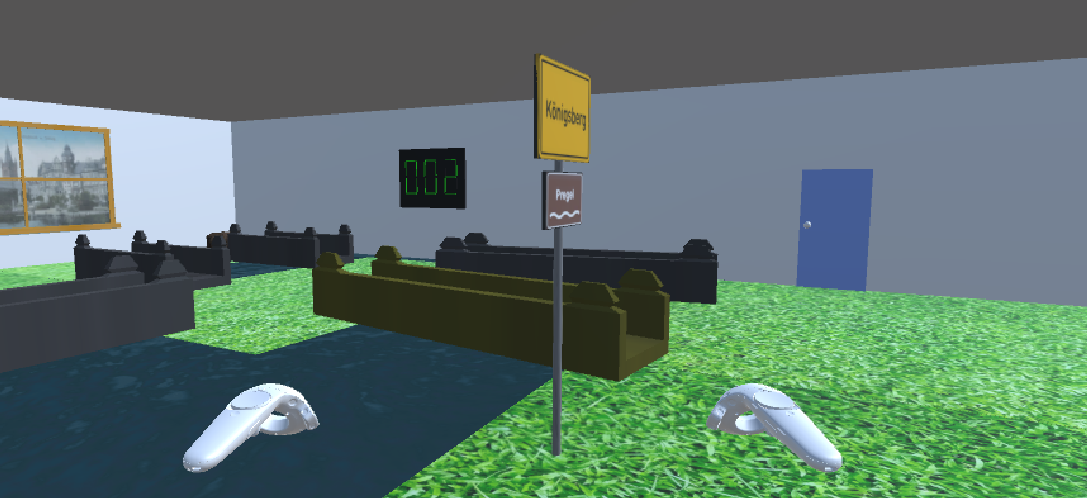
\includegraphics[width=1\textwidth]{images/neuerungen/brueckenproblem.png}
	\caption{K�nigsberger Br�ckenproblem mit ge�nderter Br�ckenfarbe (bereits benutzt) und Z�hler}
	\label{img:brueckenproblem}
\end{figure}

\begin{figure}
	\centering
	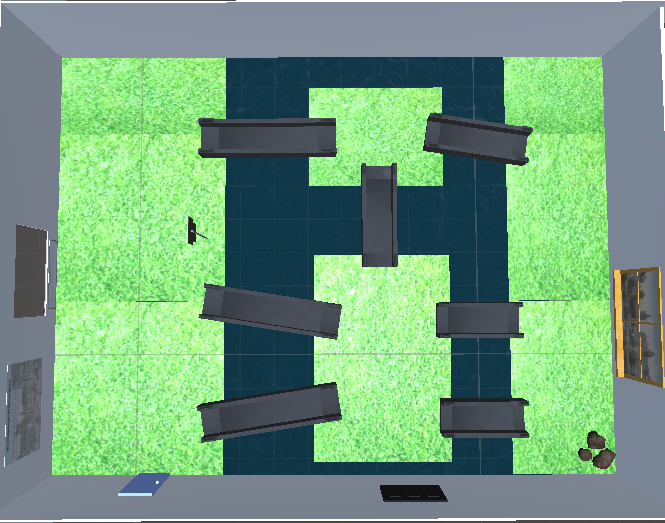
\includegraphics[width=1\textwidth]{images/neuerungen/grundriss_mathelab.png}
	\caption{Grundriss Mathematiklabor}
	\label{img:grundrissmathelab}
\end{figure}

\begin{figure}
	\centering
	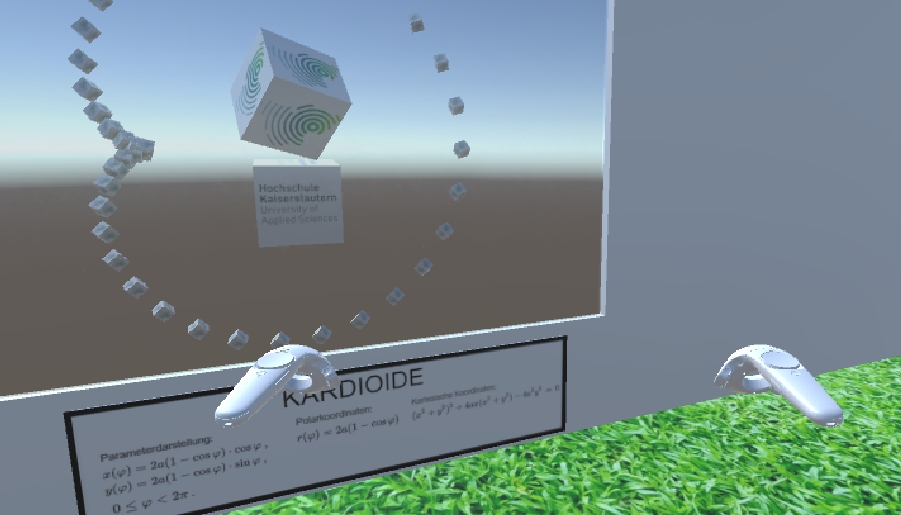
\includegraphics[width=1\textwidth]{images/neuerungen/mathelab_kardioide.png}
	\caption{Karidoide am Fenster im Raum}
	\label{img:kardioide}
\end{figure}
\begin{figure}
	\centering
	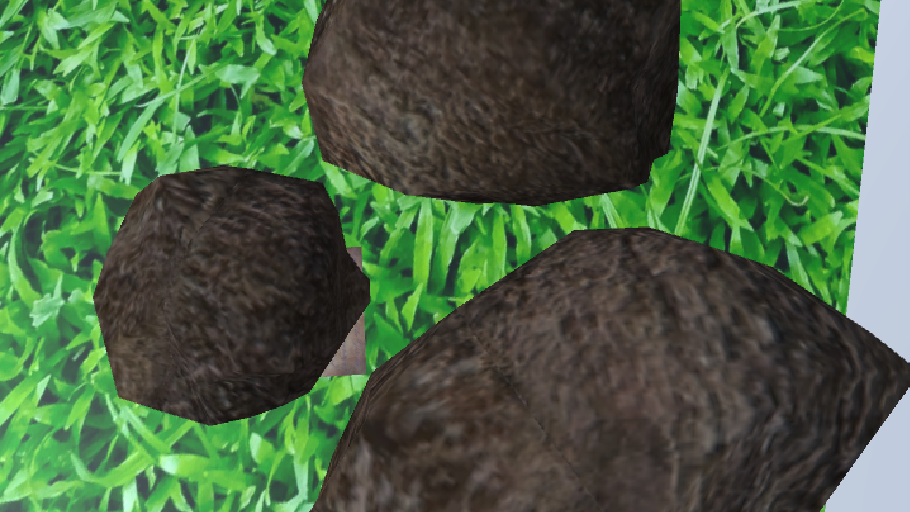
\includegraphics[width=1\textwidth]{images/neuerungen/mathelab_briefkasten.png}
	\caption{Steine im Raum als toter Briefkasten}
	\label{img:toterbriefkasten}
\end{figure}

\clearpage
\section{Informatik}
Das Informatiklabor bietet zwei Versuche, bei denen das angesprochene Problem der schwierigen Visualisierung am st�rksten aufgetreten ist. Diese sind der Suchalgorithmus Bubble Sort und der Dijkstra-Algorithmus, der den k�rzesten Weg innerhalb eines Graphen aufzeigt.  \newline

Die Wahl ist schlie�lich so ausgefallen, dass der Bubble Sort in einer Box auf einem Tisch dargestellt wird, welche mit Cubes mit zugeh�rigen Zahlenwerten gef�llt ist. Dabei werden immer zwei F�cher der Box gleichzeitig ge�ffnet, sodass man gegebenenfalls die beiden Elemente tauschen muss, falls ein kleinerer Wert rechts eines gr��eren liegt. Dies wird solange durchgef�hrt, bis alle Cubes an der richtigen Stelle platziert sind. Visuelles Feedback bekommt der User durch F�rben der Bl�cke zu gr�n, sobald sie an der richtigen Position liegen.

\begin{figure}
	\centering
	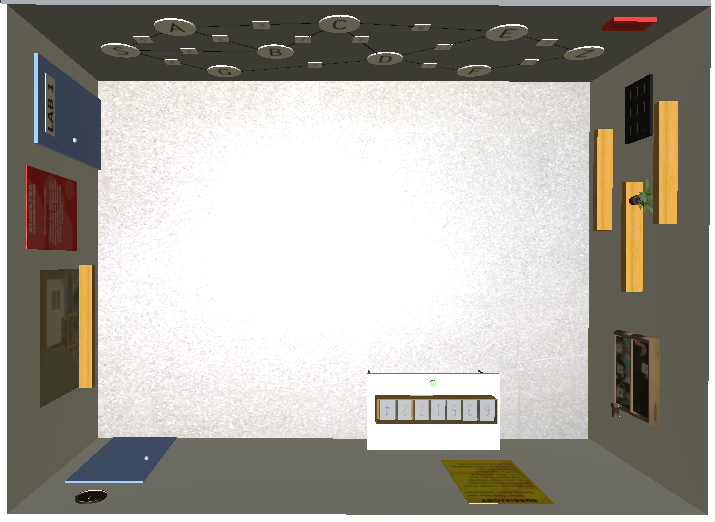
\includegraphics[width=1\textwidth]{images/neuerungen/grundriss_informatiklab.png}
	\caption{Grundriss Informatiklab}
	\label{img:informartiklab}
\end{figure}
\begin{figure}
	\centering
	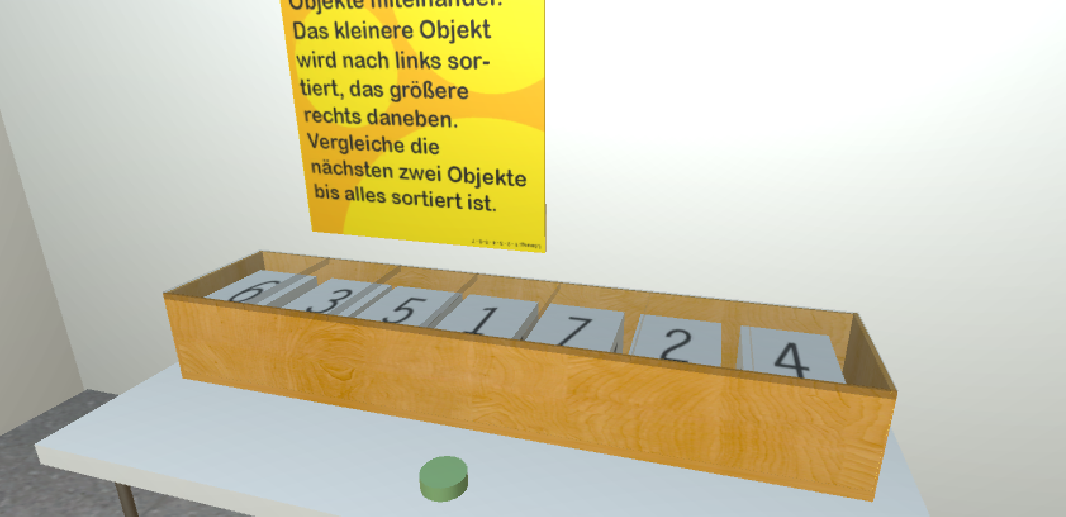
\includegraphics[width=1\textwidth]{images/neuerungen/informatiklab_bubblesort.png}
	\caption{Bubble Sort mit Button um n�chstes Fach zu �ffnen}
	\label{img:bubblesort}
\end{figure}

Der Dijkstra-Algorithmus ist an der Wand platziert und die einzelnen Knotenpunkte sind durch Ber�hrung des Controllers abzugehen. Dabei erscheint ebenso ein virtuelles Feedback. Knoten, die bereits besucht wurden, sind gr�n, m�gliche Knoten im n�chsten Schritt werden gelb hinterlegt. Ein Sieben-Segment Z�hler rechnet die Werte der abgelaufenen Pfade zusammen. Wird die Zahl rot ist man �ber den Wert des k�rzesten Weges gekommen. Erscheint sie gr�n hat man erfolgreich den k�rzesten Weg absolviert. Will man den Z�hler zur�cksetzen w�hlt man den Reset-Knopf und man kann von vorne beginnen. 

\begin{figure}
	\centering
	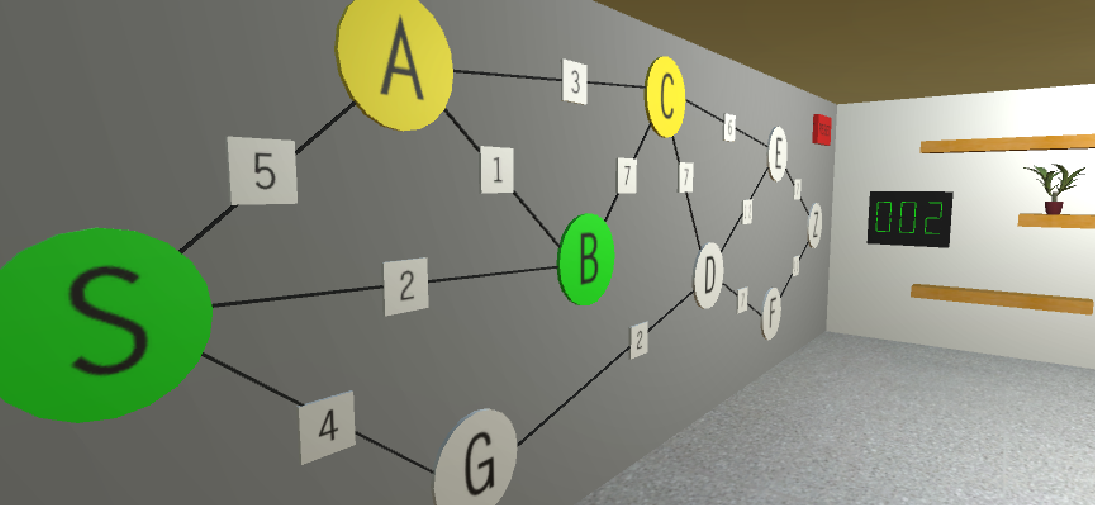
\includegraphics[width=1\textwidth]{images/neuerungen/informatiklab_dijkstra.png}
	\caption{Dijkstra-Algorithmus, gr�ne Knoten besucht, gelbe Knoten besuchbar, Z�hler und Reset-Button}
	\label{img:dijkstra}
\end{figure}

Hier sind einige seltsame Probleme aufgetreten, die sich auch im Nachhinein nicht erkl�ren lassen. Bei Tests im Simulator und mit der HTC Vive Pro kommen teils verschiedene Ergebnisse hervor. Der Bubble Sort wirft mit der Brille nach einer bestimmten Zeit einen Stack-Overflow Fehler auf, bei dem nicht klar zu erkennen ist, wieso dieser entsteht. Der Counter hat auch in beiden Ausf�hrungen verschiedene Probleme gehabt, teils ging er nur im Simulator, teils nur mit Brille, teils weder noch. Diese Probleme werden, um es leicht zu machen einfach auf kleine Bugs von der Seite von Unity oder des HTC Vive Plugins geschoben. Anders sind diese (f�r uns) nicht erkl�rbar.

\clearpage
\section{Teilchenlabor}

Das Teilchenlabor hat auf einer relativ spontanen Idee basiert und soll zeigen, wie das Verhalten von einzelnen Wassermolek�len (H\textsuperscript{2}O) bei sich ver�ndernder Raumtemperatur ist. Dazu fliegen bei Betreten des Raums die Molek�le von Wand zu Wand von denen sie sich absto�en. Auch Kollisionen miteinander f�hren zu einem Richtungswechsel. 

\begin{figure}
	\centering
	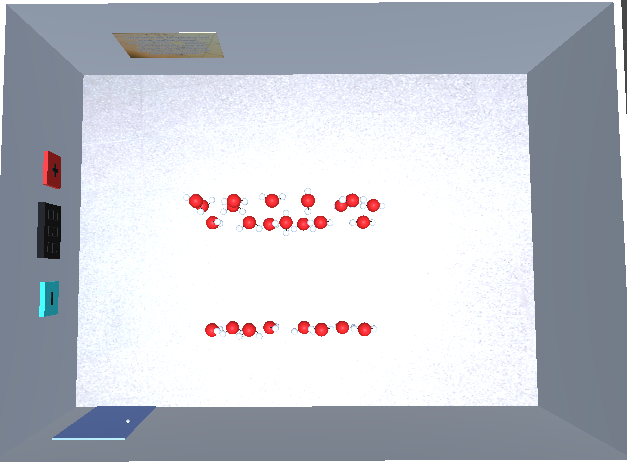
\includegraphics[width=1\textwidth]{images/neuerungen/grundriss_teilchenlab.png}
	\caption{Grundriss Teilchenlabor}
	\label{img:teilchenlab}
\end{figure}
\begin{figure}
	\centering
	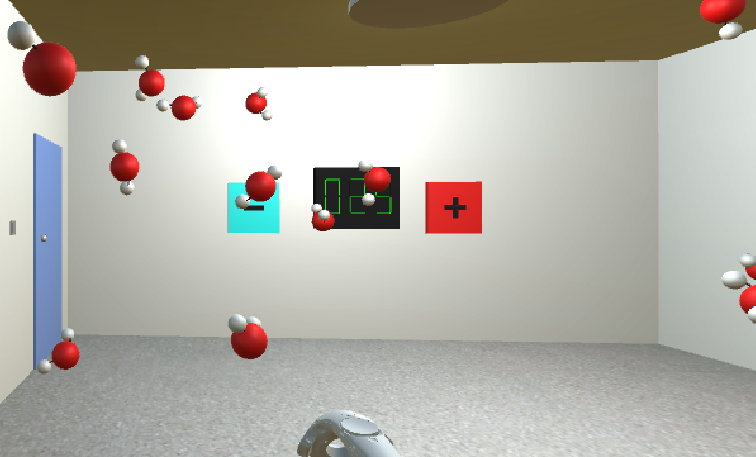
\includegraphics[width=1\textwidth]{images/neuerungen/teilchenlab_temp.png}
	\caption{Teilchenlabor mit Display und Temperatursteuerung}
	\label{img:teilchenlabtemp}
\end{figure}

Dabei hat sich als Problem herausgestellt, dass Mesh-Collider in den aktuelleren Unity-Versionen nicht mehr unterst�tzt werden, wodurch die Molek�le zu Beginn immer durch die W�nde geflogen sind und langsam, aber sicher verschwanden. Ein m�glicher L�sungsansatz war es, um das gesamte Molek�lgebilde einen Cube-Collider zu legen, sodass die Molek�le sich gegenseitig und auf die Cube-Collider des Raumes reagieren k�nnen. \newline

Ein kleineres weiteres Problem ist es, dass es ein sehr unangenehmes Gef�hl ist, wenn ein Molek�l direkt auf den User zufliegt und einen am Kopf treffen w�rde. Daf�r wurde jedoch keine passable L�sung gefunden. 

\clearpage
\section{Elektrotechnik}
Die beiden Versuche der Elektrotechnik sind raumtechnisch im Hinterzimmer des Physiklabors. Das liegt ganz einfach daher, dass ansonsten eine gerade Anzahl an R�umen im Flur entstanden w�re, was nicht aufteilbar gewesen w�re und daher wurde dies fachlich der Physik ''untergeordnet''.  \newline

Zu diesen Versuchen wurde auf tatkr�ftige Unterst�tzung von Herr Dr.-Ing. Hubert Zitt gebaut, der f�r uns die Versuche im Elektrotechnik-Labor der Hochschule Kaiserslautern in Realit�t aufgebaut hat und uns genau beschrieb, welche Vorg�nge umgesetzt werden sollen und was veranschaulicht werden soll. 

\begin{figure}
	\centering
	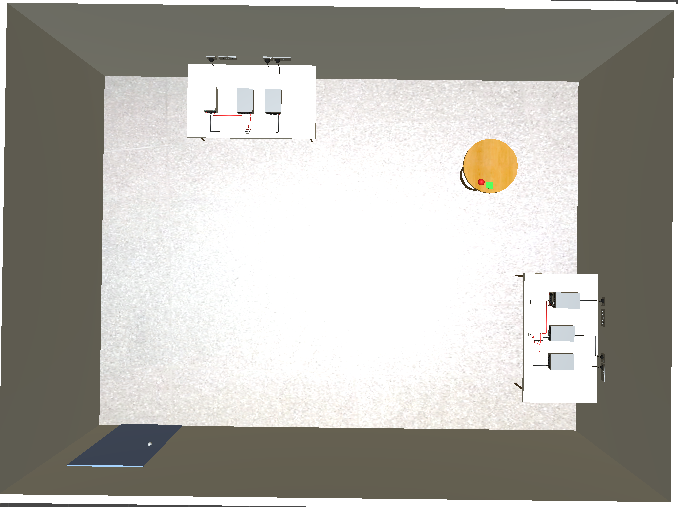
\includegraphics[width=1\textwidth]{images/neuerungen/grundriss_elektrotechnik.png}
	\caption{Grundriss Elektrotechniklabor}
	\label{img:etechniklab}
\end{figure}

Das gr��te Problem hierbei waren vor allem die Kabel in VR umzusetzen. Es w�re prinzipiell sch�ner gewesen, wenn ein User die Buchsen der Ger�te selbst verkabeln k�nnte, dies gab die Zeit und auch unsere Erfahrung mit Unity nicht her, solch ein Vorhaben w�rde den vorgegebenen Rahmen um ein Vielfaches sprengen. Daher wurde die Wahl auf statische Kabel getroffen, welche aus etlichen Zylindern einzeln zusammengebaut wurden. Ein weiteres Problem war es, an die ben�tigten Formeln heranzukommen, da es hierbei hin und wieder zu Missverst�ndnissen kam. Gel�st wurde dieses Problem durch zur Hilfenahme von Interpolation. \newline

Bei dem ersten Versuch wird Strom und Spannung bei einem nichtlinearen Verbraucher gemessen. \cite{ZittScript1} Der zweite Versuch veranschaulicht das Messen von Spannungen bei einer RC-Reihenschaltung. \cite{ZittScript2}

\begin{figure}
	\centering
	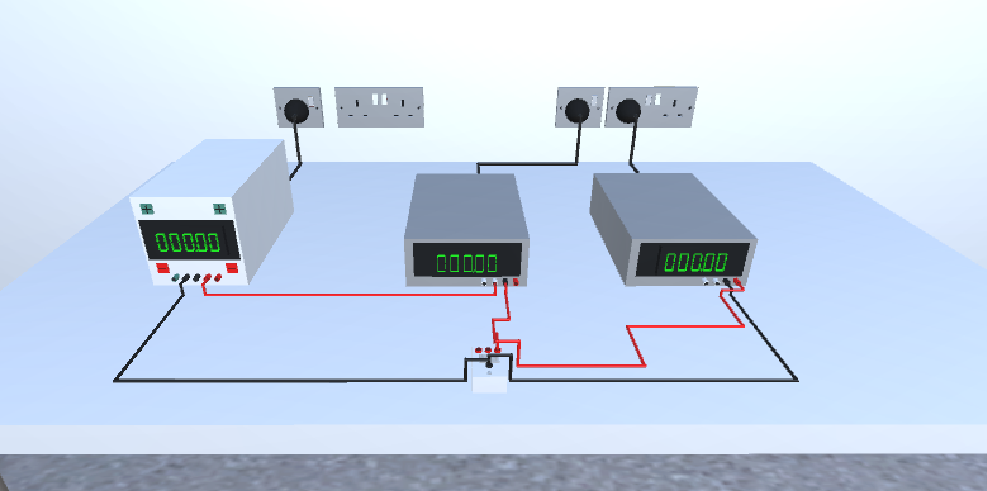
\includegraphics[width=1\textwidth]{images/neuerungen/etechnik_v1.png}
	\caption{Versuch: Messen von Strom und Spannung bei einem nichtlinearen Verbraucher}
	\label{img:etechniklabv1}
\end{figure}
\begin{figure}
	\centering
	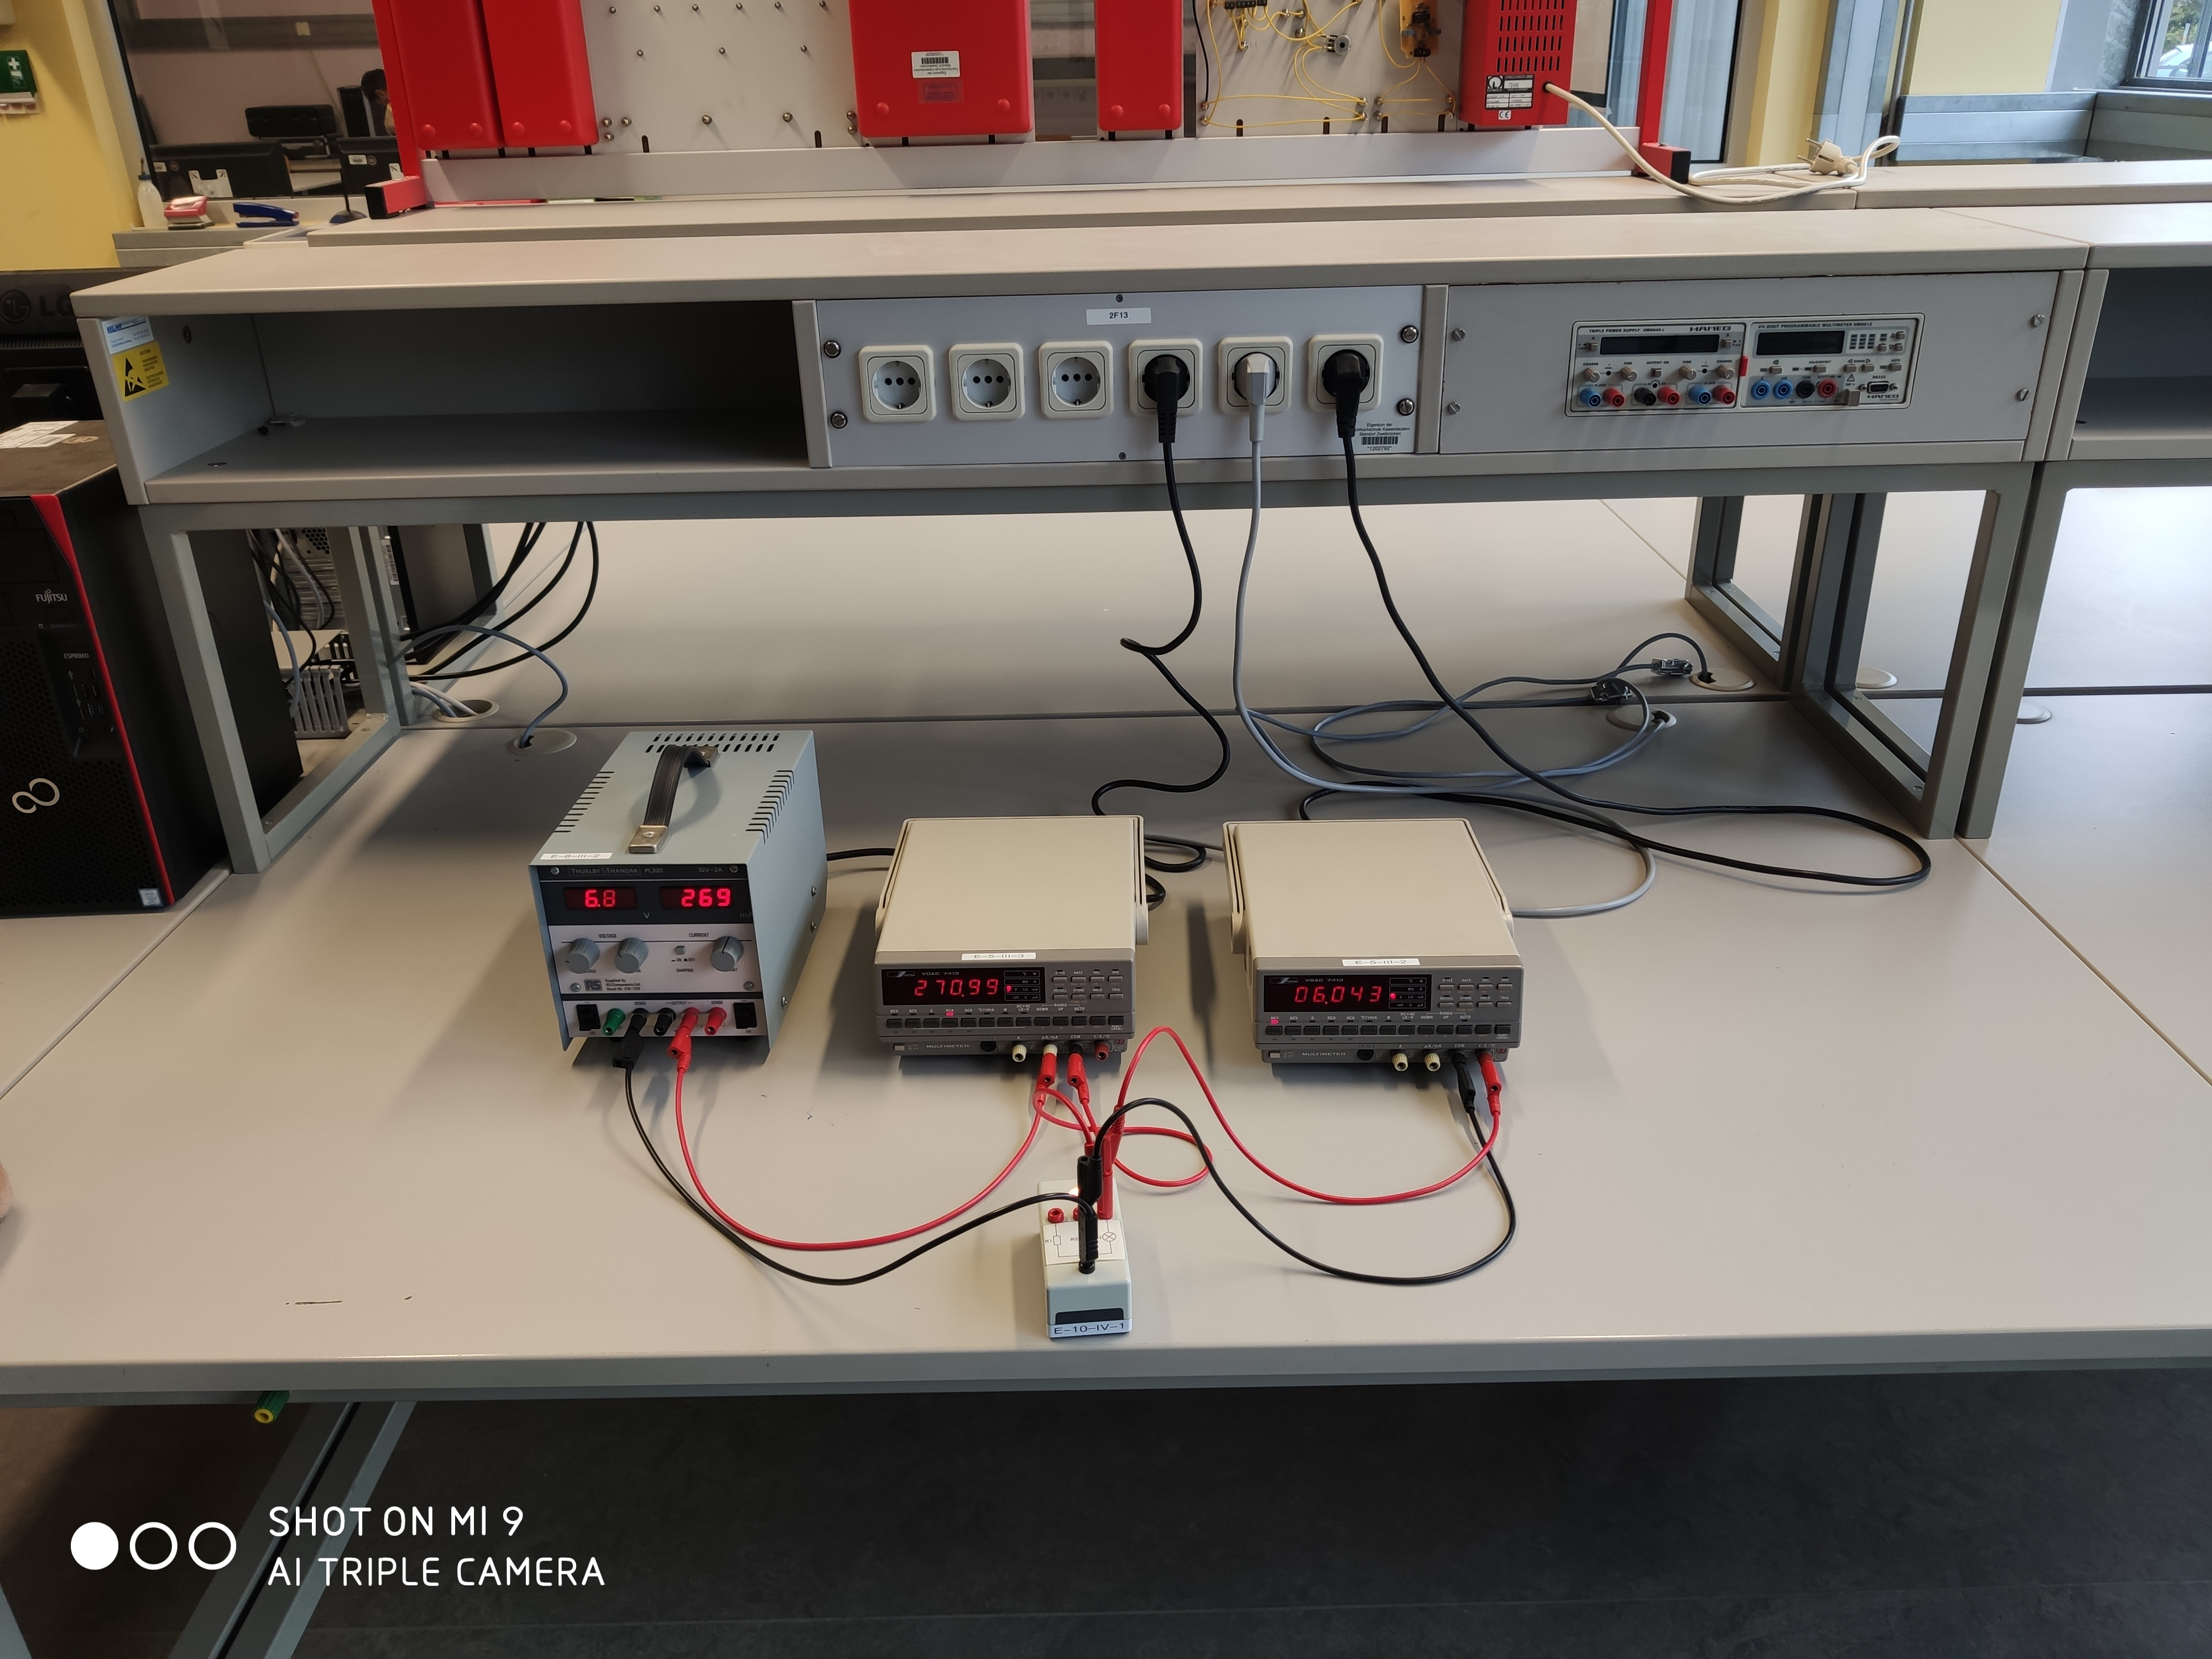
\includegraphics[width=1\textwidth]{images/neuerungen/lampe_versuchsaufbau.jpg}
	\caption{realer Versuch: Messen von Strom und Spannung bei einem nichtlinearen Verbraucher}
	\label{img:etechniklabv1real}
\end{figure}

\begin{figure}
	\centering
	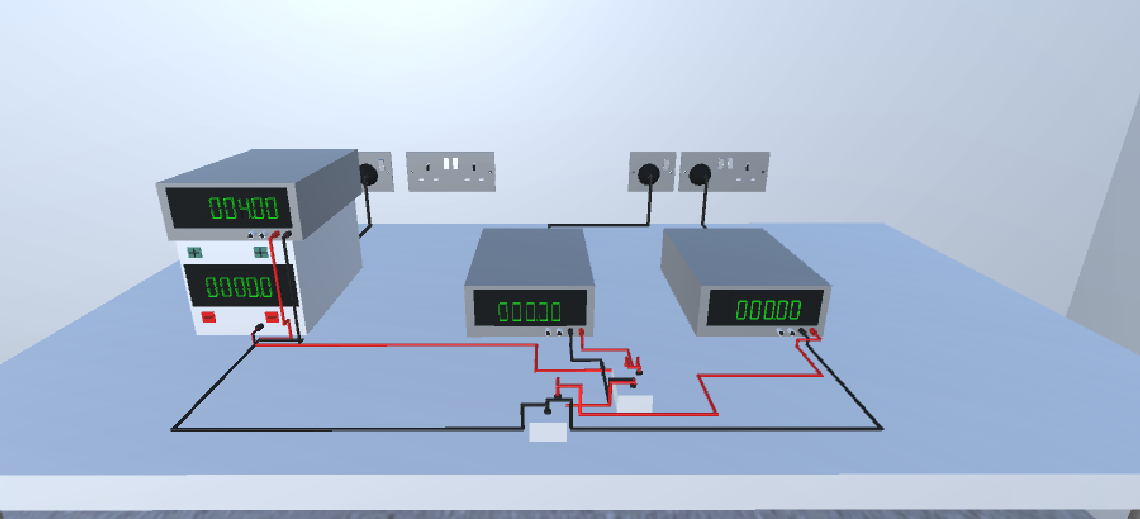
\includegraphics[width=1\textwidth]{images/neuerungen/etechnik_v2.png}
	\caption{Versuch: Messen von Spannungen bei einer RC-Reihenschaltung}
	\label{img:etechniklabv2}
\end{figure}

\begin{figure}
	\centering
	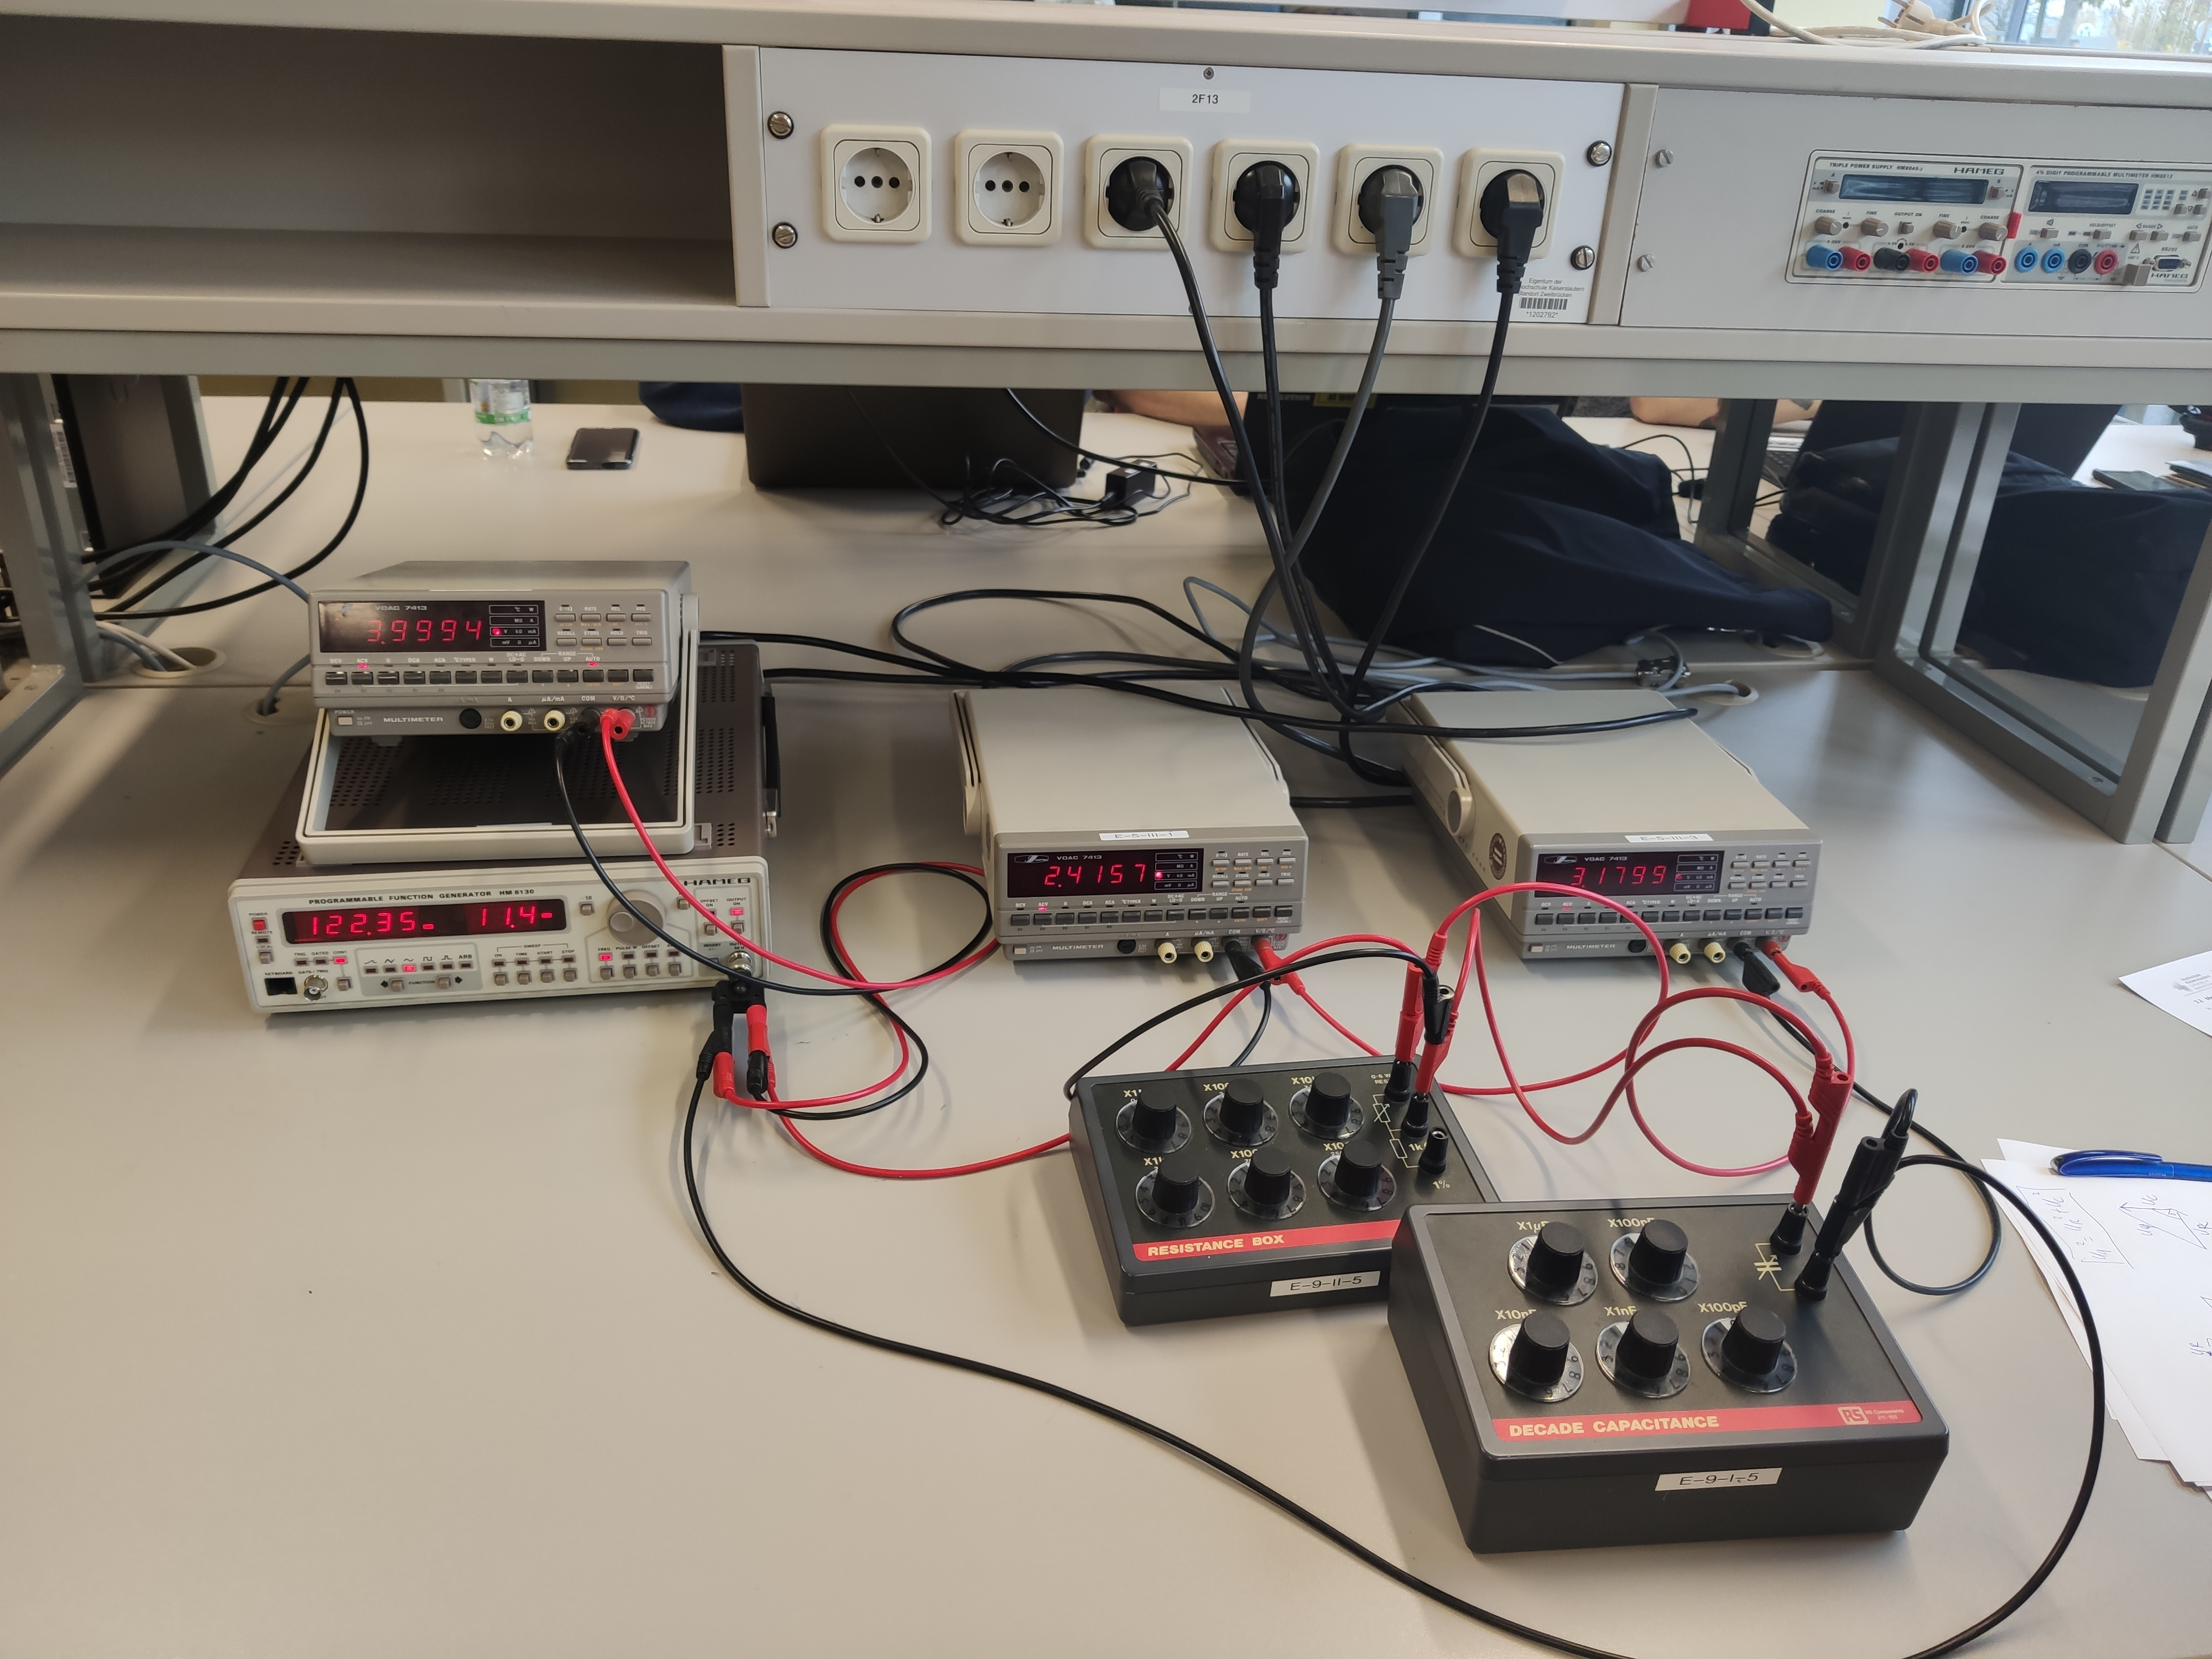
\includegraphics[width=1\textwidth]{images/neuerungen/frequenz_versuch_aufbau.jpg}
	\caption{realer Versuch: Messen von Spannungen bei einer RC-Reihenschaltung}
	\label{img:etechniklabv2real}
\end{figure}
% !TeX root = ../pythonTutorial.tex
\chapter{Code}
\section{Allgemeine Scripte}

Viele Funktionen sind in Unity standardm��ig implementiert. So zum Beispiel die M�glichkeit physikalische Eigentschaften auf ein Objekt zu definieren. Dies macht es anfassbar und erm�glicht die Interaktion mit dem Objekt. \newline

Eigene bzw. weitere und schwierigere Funktionen m�ssen hingegen selbst implementiert werden. Alle von uns implementierten Funktionen und Methoden befinden sich im Projekt unter Assets -> Scripts. Alle Scripte wurden in C# programmiert. \newline

Es gibt Scripte, die sich durchs ganze Projekt ziehen und andere, die sich auf bestimmte Szenen beziehen. Allgemein k�nnen jedoch alle Scripte �berall verwendet werden.

\clearpage
\subsection{Scene\_Management.cs}

Das Scene Management Script dient zur richtigen Positionierung des Spielers, wenn er den Flur betritt. Je nachdem aus welchem Raum er kommt �ndert sich die Startposition. Das Script muss in jeder Szene eingebaut sein, da nur so die zuletzt verwendete Szene ausgelesen werden kann. 

\begin{lstlisting}
Scene scene = SceneManager.GetActiveScene();
camera_obj = GameObject.Find("ViveRig");
Vector3 vec = new Vector3();

if (scene.name == "NeuerFlur" && Globals.last_scene != "")
{
Debug.Log("Switching Cam from: " + Globals.last_scene);
switch (Globals.last_scene)
{
case "BioLab":
vec = new Vector3(12.0f, 0f, -1.4f);
break;
case "grosserRaum": // Mathe
vec = new Vector3(9.2f, 0f, 0f);
break;
case "Lab1": // Chemie
vec = new Vector3(22.0f, 0f, -1.4f);
break;
case "Lab2": // Physik
vec = new Vector3(22.0f, 0f, 1.4f);
break;
case "Lab3": // Informatik
vec = new Vector3(16.9f, 0f, 1.4f);
break;
case "Teilchenlabor":
vec = new Vector3(12.0f, 0f, 1.4f);
break;
case "VRLab":
vec = new Vector3(16.9f, 0f, 1.4f);
break;
}
Debug.Log("Changing Position: " + vec);
camera_obj.transform.position = vec;
} else
{
Globals.last_scene = scene.name;
}
\end{lstlisting}

Das Script wird in der \textit{start()} Methode ausgef�hrt - also beim Laden der Szene. Am Anfang wird der Szenenname rausgefunden und in einer Variable gespeichert. Anschlie�end erfolgt eine Abfrage, ob die aktuelle Szene der "Flur" ist oder nicht. Falls nicht, wird der aktuelle Scenenname als \textit{last\_scene} in einer Globalen Variable gespeichert. Wenn es sich um den Flur handelt wird die Position des Players entsprechend der letzten Szene im Flur ge�ndert.

\clearpage
\subsection{Globals.cs}

In der Globals.cs werden globale Variablen gespeichert, die Szenen�bergreifend ben�tigt werden. Aktuell ist dies nur der letzte Szenenname.

\begin{lstlisting}
public static class Globals {

public static string last_scene = "";
}
\end{lstlisting}

\clearpage
\subsection{Load\_publics.cs}

In diesem Script werden alle Variablen gespeichert, die �ber ein Script hinaus aber nur innerhalb einer Szene ben�tigt werden. Das Script wird in jeder Szene eingebunden. Das Objekt auf dem es positioniert ist, spielt dabei keine Rolle. \newline

\begin{lstlisting}
//Allgemein
public static bool light_on = false;
public static bool light_col = false;
public static string[] lightnames = {"Point_Light_l", 
"Point_Light_m", "Point_light_r"};

// Informatiklab
// Dijkstra
internal static readonly bool reset_clicked;
public static string Dijkstra_Word;
public static bool s_active = true;
public static bool a_active = false;
public static bool b_active = false;
public static bool g_active = false;
public static bool c_active = false;
public static bool d_active = false;
public static bool e_active = false;
public static bool f_active = false;
public static bool z_active = false;
public static bool r_active = false;

public static bool s_clicked = false;
public static bool a_clicked = false;
public static bool b_clicked = false;
public static bool g_clicked = false;
public static bool c_clicked = false;
public static bool d_clicked = false;
public static bool e_clicked = false;
public static bool f_clicked = false;
public static bool z_clicked = false;
public static bool r_clicked = false;

public static int counter = 0;
public static int maximum = 19;
public static string last_clicked = "";


// Bubblesort
public static int b_state = 0;
public static bool bubble_active = true;
public static bool s_1_act = true;
public static bool s_2_act = true;
public static bool s_3_act = true;
public static bool s_4_act = true;
public static bool s_5_act = true;
public static bool s_6_act = true;
public static bool s_7_act = true;

// BioLab
public static string scene_change = "";
public static bool bio_collision_happened = false;

// Teilchenlabor
// Molekuele
public static int Temperatur = 25;
public static bool min_act = true;
public static bool plus_act = true;
public static float Temp_Max = 200f;
public static float Temp_Min = 0f;
public static float Map_Temp_Max = 0.25f;
public static float Map_Temp_Min = 0f;
public static float move_speed_multi = 15;
public static float RemapTemp(float from, float fromMin, 
float fromMax, float toMin, float toMax)
{
var fromAbs = from - fromMin;
var fromMaxAbs = fromMax - fromMin;
var normal = fromAbs / fromMaxAbs;
var toMaxAbs = toMax - toMin;
var toAbs = toMaxAbs * normal;
var to = toAbs + toMin;

return to;
}

// Mathelab
public static int sev_bridges_counter = 0;
public static bool bridges_active = true;

// Elektrolab
public static double lampe_netzteil_count = 0;
public static float RemapLight(float from, float fromMin, 
float fromMax, float toMin, float toMax)
{
var fromAbs = from - fromMin;
var fromMaxAbs = fromMax - fromMin;
var normal = fromAbs / fromMaxAbs;
var toMaxAbs = toMax - toMin;
var toAbs = toMaxAbs * normal;
var to = toAbs + toMin;

return to;
}

// Versuch 2
public static float Uq = 4.0f;
public static float R = 2000f;
public static float C = 0.5f;
public static float frequency_Netzteil = 0.0f;
\end{lstlisting}

Wichtig ist, dass in dem Script eine Klasse definiert ist, die die Variablen und f�r die Variablen wichtige Funktionen z. B. zum Mapping von manchen Variablen enth�lt.

\clearpage
\subsection{Sev\_Seg\_counter.cs}

Die 7-Segment-Anzeige wird in verschiedenen Szenen benutzt. Dieses Script dient dazu eine eingegebenen Zahl auf das 3-Ziffern-Display zu �bertragen. \newline
Der Funktion \textit{setSevSegCount()} wird eine Zahl als int und der Name des zugeh�rigen Parent-Objekts �bergeben. Die Zahl wird als String formatiert, sodass sie besser in 3 Teile geteilt werden kann. Das Parent-Objekt wird per \textit{Find} Befehl gesucht und in einer Variable gespeichert. Anschlie�end wird f�r jede der 3 Zeichen des Zahl-Strings die Funktion \textit{set\_n()} aufgerufen, welche die entsprechende Position in der 7-Segment-Anzeige in die Zahl umwandelt. \newline

Innerhalb der \textit{set\_n()} Methode werden die Segment-Objekte innerhalb des Parent-Objekts gesucht. Da die Benennung immer gleich ist, kann dies programmatisch anhand eines zusammengesetzten Strings geschehen. Anschlie�end wird f�r jedes Segment der Anzeige die Farbe entsprechend einer Vorgabe, die per If-Abfrage anhand der eingegebenen Zahl festgestellt wird, entweder Schwarz oder Rot bzw. Gr�n gesetzt. Dadurch entsteht die Zahl auf der Anzeige.

\begin{lstlisting}
public void setSevSegCount(int seconds, String parentname)
{
if (seconds < 1000)
{
string s_number = String.Format("{0:000}", seconds);
GameObject parent = GameObject.Find(parentname);

Debug.Log(s_number);

set_n(int.Parse(Char.ToString(s_number[0])), 1, parent);
set_n(int.Parse(Char.ToString(s_number[1])), 2, parent);
set_n(int.Parse(Char.ToString(s_number[2])), 3, parent);
}
}

private void set_n(int number, int disp_num, 
GameObject parent_item)
{
string s_lt = "n_" + disp_num + "_lt";
string s_rt = "n_" + disp_num + "_rt";
string s_lb = "n_" + disp_num + "_lb";
string s_rb = "n_" + disp_num + "_rb";
string s_m = "n_" + disp_num + "_m";
string s_b = "n_" + disp_num + "_b";
string s_t = "n_" + disp_num + "_t";

Debug.Log(parent_item);
Debug.Log(number);

switch (number)
{
case 0:
setColorP(parent_item.transform.Find(s_lt).gameObject);
setColorP(parent_item.transform.Find(s_rt).gameObject);
setColorP(parent_item.transform.Find(s_lb).gameObject);
setColorP(parent_item.transform.Find(s_rb).gameObject);
setColorN(parent_item.transform.Find(s_m).gameObject);
setColorP(parent_item.transform.Find(s_b).gameObject);
setColorP(parent_item.transform.Find(s_t).gameObject);
break;
case 1:
setColorN(parent_item.transform.Find(s_lt).gameObject);
setColorP(parent_item.transform.Find(s_rt).gameObject);
setColorN(parent_item.transform.Find(s_lb).gameObject);
setColorP(parent_item.transform.Find(s_rb).gameObject);
setColorN(parent_item.transform.Find(s_m).gameObject);
setColorN(parent_item.transform.Find(s_b).gameObject);
setColorN(parent_item.transform.Find(s_t).gameObject);
break;
case 2:
setColorN(parent_item.transform.Find(s_lt).gameObject);
setColorP(parent_item.transform.Find(s_rt).gameObject);
setColorP(parent_item.transform.Find(s_lb).gameObject);
setColorN(parent_item.transform.Find(s_rb).gameObject);
setColorP(parent_item.transform.Find(s_m).gameObject);
setColorP(parent_item.transform.Find(s_b).gameObject);
setColorP(parent_item.transform.Find(s_t).gameObject);
break;
case 3:
setColorN(parent_item.transform.Find(s_lt).gameObject);
setColorP(parent_item.transform.Find(s_rt).gameObject);
setColorN(parent_item.transform.Find(s_lb).gameObject);
setColorP(parent_item.transform.Find(s_rb).gameObject);
setColorP(parent_item.transform.Find(s_m).gameObject);
setColorP(parent_item.transform.Find(s_b).gameObject);
setColorP(parent_item.transform.Find(s_t).gameObject);
break;
case 4:
setColorP(parent_item.transform.Find(s_lt).gameObject);
setColorP(parent_item.transform.Find(s_rt).gameObject);
setColorN(parent_item.transform.Find(s_lb).gameObject);
setColorP(parent_item.transform.Find(s_rb).gameObject);
setColorP(parent_item.transform.Find(s_m).gameObject);
setColorN(parent_item.transform.Find(s_b).gameObject);
setColorN(parent_item.transform.Find(s_t).gameObject);
break;
case 5:
setColorP(parent_item.transform.Find(s_lt).gameObject);
setColorN(parent_item.transform.Find(s_rt).gameObject);
setColorN(parent_item.transform.Find(s_lb).gameObject);
setColorP(parent_item.transform.Find(s_rb).gameObject);
setColorP(parent_item.transform.Find(s_m).gameObject);
setColorP(parent_item.transform.Find(s_b).gameObject);
setColorP(parent_item.transform.Find(s_t).gameObject);
break;
case 6:
setColorP(parent_item.transform.Find(s_lt).gameObject);
setColorN(parent_item.transform.Find(s_rt).gameObject);
setColorP(parent_item.transform.Find(s_lb).gameObject);
setColorP(parent_item.transform.Find(s_rb).gameObject);
setColorP(parent_item.transform.Find(s_m).gameObject);
setColorP(parent_item.transform.Find(s_b).gameObject);
setColorP(parent_item.transform.Find(s_t).gameObject);
break;
case 7:
setColorN(parent_item.transform.Find(s_lt).gameObject);
setColorP(parent_item.transform.Find(s_rt).gameObject);
setColorN(parent_item.transform.Find(s_lb).gameObject);
setColorP(parent_item.transform.Find(s_rb).gameObject);
setColorN(parent_item.transform.Find(s_m).gameObject);
setColorN(parent_item.transform.Find(s_b).gameObject);
setColorP(parent_item.transform.Find(s_t).gameObject);
break;
case 8:
setColorP(parent_item.transform.Find(s_lt).gameObject);
setColorP(parent_item.transform.Find(s_rt).gameObject);
setColorP(parent_item.transform.Find(s_lb).gameObject);
setColorP(parent_item.transform.Find(s_rb).gameObject);
setColorP(parent_item.transform.Find(s_m).gameObject);
setColorP(parent_item.transform.Find(s_b).gameObject);
setColorP(parent_item.transform.Find(s_t).gameObject);
break;
case 9:
setColorP(parent_item.transform.Find(s_lt).gameObject);
setColorP(parent_item.transform.Find(s_rt).gameObject);
setColorN(parent_item.transform.Find(s_lb).gameObject);
setColorP(parent_item.transform.Find(s_rb).gameObject);
setColorP(parent_item.transform.Find(s_m).gameObject);
setColorP(parent_item.transform.Find(s_b).gameObject);
setColorP(parent_item.transform.Find(s_t).gameObject);
break;
}
}

private void setColorP(GameObject gameObject)
{
if(Load_Publics.counter <= Load_Publics.maximum)
{
gameObject.GetComponent<Renderer>().material.color 
= Color.green;
} else
{
gameObject.GetComponent<Renderer>().material.color 
= Color.red;
}

}
private void setColorN(GameObject gameObject)
{
gameObject.GetComponent<Renderer>().material.color 
= Color.black;
}

}
\end{lstlisting}

\clearpage
\subsection{Display\_Meter\_5D.cs}

�hnlich des Scripts \textit{Sev\_Seg\_counter.cs} ist auch dieses Script zum Anzeigen von Zahlen auf einer 7-Segment-Anzeige gedacht. Die Besonderheit hier ist, dass 5 Ziffern dargestellt werden und die letzten beiden Ziffern nach einem Komma stehen. Also eine Kommazahl. \newline

Der Unterscheid der beiden Scripte besteht rein in der Formatierung der Zahl und der Eingabe einer Double-Variable, anstatt einer Integer-Variable. Der Rest ist identisch. Einzig die \textit{set\_n()}-Methode wird f�nf mal anstatt nur drei mal aufgerufen.

\begin{lstlisting}
public void setDisplay(double do_number, string parent_name)
{
if(do_number < 1000)
{
string s_number = String.Format("{0:000.00}", do_number);
GameObject parent = GameObject.Find(parent_name);

Debug.Log(s_number);

set_n(int.Parse(Char.ToString(s_number[0])), 1, parent);
set_n(int.Parse(Char.ToString(s_number[1])), 2, parent);
set_n(int.Parse(Char.ToString(s_number[2])), 3, parent);
set_n(int.Parse(Char.ToString(s_number[4])), 4, parent);
set_n(int.Parse(Char.ToString(s_number[5])), 5, parent);

setColorP(parent.transform.Find("decimal_point").gameObject);
}
}
\end{lstlisting}

\clearpage
\section{Szenenspezifische Scripte}
\subsection{Beschleunigung.cs}

Dieses Script ist f�r die Steuerung der Geschwindigkeit der Teilchen im Teilchenlabor zust�ndig.

\begin{lstlisting}
public class Beschleunigung : MonoBehaviour {


// Use this for initialization
void Start () {
Sev_Seg_Counter counti = new Sev_Seg_Counter();
counti.setSevSegCount(0, "Z�hler1");
}

// Update is called once per frame
void Update () {
Sev_Seg_Counter counti = new Sev_Seg_Counter();
counti.setSevSegCount(Load_Publics.Temperatur, "Z�hler1");
}

private void OnTriggerEnter(Collider other)
{
switch (gameObject.name)
{
case "plus":
if (Load_Publics.plus_act && Load_Publics.Temperatur 
< Load_Publics.Temp_Max)
{
Load_Publics.Temperatur += 25;
Debug.Log("w�rmer");
StartCoroutine(waiter(true));
}
break;
case "minus":
if (Load_Publics.min_act && Load_Publics.Temperatur 
> Load_Publics.Temp_Min)
{
Load_Publics.Temperatur -= 25;
Debug.Log("k�lter");
StartCoroutine(waiter(false));
}
break;
}
}

IEnumerator waiter(bool isplus)
{
GameObject button_mol = null;
if (isplus)
{
button_mol = GameObject.Find("plus");
Load_Publics.plus_act = false;
} else
{
button_mol = GameObject.Find("minus");
Load_Publics.min_act = false;
}
button_mol.GetComponent<Renderer>().material.color 
= Color.yellow;

yield return new WaitForSeconds(1);    //Wait 1 Second
Color color = new Color();

if (isplus)
{
Load_Publics.plus_act = true;
if(ColorUtility.TryParseHtmlString("#FF0000", out color))
{
button_mol.GetComponent<Renderer>().material.color = color;
}
}
else
{
Load_Publics.min_act = true;
if (ColorUtility.TryParseHtmlString("#00FFFF", out color))
{
button_mol.GetComponent<Renderer>().material.color = color;
}
}
}
}
\end{lstlisting}

Das Script wurde auf die beiden Buttons in der Szene zum Beschleunigen und Abbremsen der Teilchen gelegt. Bei Aufruf der Szene wird zuerst in der \textit{start()} die 7-Segment-Anzeige auf 0 gesetzt. Das ist der Temperatur Startwert. Anschlie�end wird die Anzeige in der \textit{Update()} jeweils auf den Wert der Temperatur-Variable in der \textit{Load\_Publics.cs} gesetzt. Standardm��ig ist dies 25. \newline

Das Script enth�lt au�erdem Listener, die ausgel�st werden, sobald der Spieler einen der Buttons ber�hrt. Diese Listener unterscheiden dann welcher Button gedr�ckt wurde und �ndern entsprechend die Temperatur-Variable. Nachdem ein Button gedr�ckt wurde wird es f�r eine Sekunde unm�glich diesen nochmals zu dr�cken. Dies wird auch durch eine Farb�nderung dargestellt.
% !TeX root = ../pythonTutorial.tex
\chapter{Interpolation}

Die Interpolation betrifft die Werte f�r die Versuche im Elektrolabor. \newline

Das Problem hier war die Beschaffung der Formeln zur Berechnung m�glichst Realistischer Werte. Die f�r den Moment einfachste Variante schien uns die reellen Zahlen in einen Graph umzuwandeln und zu schauen welche Funktion m�glichst nah ran kommt.

\section{Frequenz-Versuch}

\section{Lampen-Versuch}
% !TeX root = ../pythonTutorial.tex
\chapter{Verworfene Ideen}

Einige Versuche und Ideen, die zu Beginn gemacht wurden, wurden letztendlich verworfen, da stattdessen andere Ideen und Inputs kamen, denen stattdessen nachgegangen wurden. Dies ist aus unserer Sicht bei einem solch flexiblen Projekt unvermeidlich. \newline

Dazu z�hlt ein Geografie Labor, f�r das bis zum Schluss keine sinnvollen Ideen gesammelt werden konnten. Zwar war die �berlegung irgendwie eine Karte mit einflie�en zu lassen, jedoch konnte keine fertige Durchf�hrung in einem Versuch konstruiert werden. \newline

Des Weiteren wurden viele Versuchsskizzen verworfen, da andere Ideen vorgezogen wurden. So zum Beispiel w�re eine Turing Maschine im Informatiklabor vorstellbar, das Sezieren eines Frosches oder Fisches im Biologielabor, so wie viele Ideen, f�r das Labor der Mathematik, wie Kugelkoordinaten. Nat�rlich kennen die Wissenschaft und somit auch das Virtual Science Lab keinen Endzustand. Es ist stets erweiterbar und durch weitere Versuche, Laborr�ume und Erweiterungen fortf�hrbar. Neben den genannten Versuchen, die es in die konkrete Ideenfindung geschafft haben, zeigt der Ausblick wie es mit dem Projekt weitergehen k�nnte. 
% !TeX root = ../pythonTutorial.tex
\chapter{Verworfene Ideen}

 Ob und wie es mit dem Projekt Virtual Science Lab weitergehen wird, steht zum Zeitpunkt dieser Abgabe noch in den Sternen, jedoch ist es von unserer Seite mehr als w�nschenswert, dass es eine Zukunft f�r das Projekt geben wird. Die aktuellen Versuche sind immer verbesserbar. Allein der Unterschied zwischen dem Bunsenbrenner im Ausgangsprojekt und der neu modellierte zeigen, dass kleine Details einen immensen Unterschied f�r das Gesamterlebnis beitragen k�nnen. Zwar wurde schon sehr auf Details wert gelegt, doch perfekt ist eben doch zuletzt im Ermessen des Betrachters. \newline
 
 Au�erdem ist es sinnvoll, den Android Build erneut anzugehen. Bei diesem besteht das gro�e Problem, verschiedene Ger�te mit unterschiedlichsten Steuerungsarten mit einzubeziehen.  \newline
 
 Au�erdem w�re eine Art Feldtest sinnvoll, in dem getestet wird, ob Sch�ler oder Studenten, die das Virtual Science Lab absolvieren, in einer passenden Pr�fung besser abschneiden k�nnten, als eine Gruppe, die das Labor nicht gesehen hat.  \newline
 
 Der Aufbau der Laborr�ume glich immer mehr einem Prozess, bei dem dieselben Schritte nacheinander abgespult wurden. Zun�chst wird der Raum durch W�nde, Boden und Decke begrenzt, eine T�r wird hinzugef�gt, vor der die Kamera platziert wird, sodass man an der Position der T�r den Raum betritt. Anschlie�end werden falls n�tig Tische angeordnet, so wie die verschiedenen Utensilien die f�r die vorgesehenen Versuche n�tig sind. Zum Schluss werden die Skripte zur Funktionalit�t geschrieben, um so die Versuchsdurchf�hrung zu erm�glichen. Anschlie�end wird der Versuch im Virtual Reality Labor getestet und falls n�tig Bugs notiert, die im Anschluss gefixt werden. Dieser Evaluationsvorgang wird iterativ beliebig oft durchgef�hrt, bis das Ergebnis zufriedenstellend ist.  \newline
 
 
% !TeX root = ../pythonTutorial.tex
\chapter{Verworfene Ideen}

Wie schon aus verschiedenen anderen Projekten hat die Zusammenarbeit problemlos funktioniert und Absprachen sowie regelm��ige Treffen im Virtual Reality Labor wurden �ber den gesamten Projektverlauf hinweg gepflegt. Alle Probleme waren nach und nach gut l�sbar und es wurde innerhalb des Projektverlaufes einiges in gegenseitigem Einverst�ndnis ge�ndert, was jedoch im Nachhinein immer eine gute Entscheidung war. Der einzige Wermutstropfen ist der zu kurz gekommene Android Build, f�r den am Ende die Zeit ausging. Zwar ist eine Ausf�hrung �ber Android Ger�te wie die Samsung VR Gear prinzipiell m�glich, allerdings ist die Steuerung der HTC Vive Pro nicht kompatibel mit solchen Low Budget Modellen. Diese Aufgabenstellung, sowie eine Evaluierung im Schul- oder Hochschulumfeld sind Dinge, die f�r die Zukunft des Projektes denkbar sind und einen n�chsten Schritt bilden sollten. \newline

Wir sind sehr froh, dass wir nun �ber einen Zeitraum von fast einem Jahr (mit dem vorherigen Semester zusammen) an dem Projekt arbeiten durften, was uns einen tiefen Einblick in die Entwicklung von Virtual Reality Anwendungen, vor allem in der Entwicklungsumgebung Unity vermitteln konnte. Auch die Erfahrungen im Arbeiten mit Git konnte deutlich verbessert werden, was mittlerweile kein Problem mehr f�r einen guten Arbeitsfluss aufgeworfen hat.  \newline

Das alleinige Ausarbeiten von Ideen, unterst�tzt von Herr Prof. Dr. Manfred Brill konnte uns jedoch vor allem tiefe Einblicke bieten, wie es ist, an einem dynamischen Projekt von  der Planung bis zur Entwicklung teilzuhaben, was uns f�r unsere sp�tere Karriere noch von gro�em Nutzen sein kann. Dabei waren auf die aufgetretenen Fehler und Probleme eine gro�e Hilfe, denn die Realit�t der Projektdurchf�hrung ist (wohl fast) nie wie die Vorstellung und Planung. \newline

Abschlie�end gilt unser Dank Herrn Prof. Dr. Brill, sowie Fabian Kalweit, die auch kurzfristig stets Zeit gefunden haben, um mit uns den weiteren Ablauf zu besprechen und auch etliche Ideen mit auf den Weg gegeben haben. Au�erdem sind wir sehr dankbar f�r die Modelle des Mikroskops und des Bunsenbrenners unseres Kommilitonen Cedric Schug, der falls der Unity Asset Store nicht ergiebig war unter die Arme gegriffen hat. Zu guter Letzt auch noch danke an Herr Dr.-Ing. Hubert Zitt, der sich ebenfalls viel Zeit nahm, um uns die beiden Elektrotechnik-Versuche genau aufzubauen, zu zeigen und zu erkl�ren. 

%
% Literatur
%
\cleardoublepage
\phantomsection
\addcontentsline{toc}{chapter}{Literaturverzeichnis}
\chaptermark{Literaturverzeichnis}
\sectionmark{Literatur}\label{literatur}
\bibliography{./bib/literatur}
\addcontentsline{toc}{chapter}{Abbildungsverzeichnis}
\chaptermark{Abbildungsverzeichnis}
\sectionmark{Abbildungsverzeichnis}
\listoffigures 

%
% Index
%\clearevenpage
%\phantomsection
%\small
%\chaptermark{Index}
%\sectionmark{Index}
%\printindex
%\normalsize
\end{document}
